\label{ch:galerkin}

\section{Introduction}

We consider a two-dimensional correlated Brownian motion:
\begin{align}
  X(t) &= x_0 + \mu_x t + \sigma_x W_x(t)  \label{eq:X} \\
  Y(t) &= y_0 + \mu_y t + \sigma_y W_y(t)  \label{eq:Y}
\end{align}
where $W_i$ are standard Brownian motions with
$\mbox{Cov}(W_1(t), W_2(t)) = \rho t$. Our interest is in finding the
joint probability density function for the pair $(X(t), Y(t))$
along with the random variables $M_X(t)=\max_{0\leq s\leq t}X(t),$
$m_X(t)=\min_{0\leq s\leq t}X(t),$ $M_Y(t)=\max_{0\leq s\leq t}Y(t),$
$m_Y(t)=\min_{0\leq s\leq t}Y(t)$
\begin{multline}
  \lim_{dy \to 0} \lim_{dx \to 0} \frac{1}{dx dy} \mbox{Pr}\left(x \leq X(t) < x+dx, y \leq Y(t) < y+dy, \right. \\
  \left. M_x(t) \leq b_x, M_y(t) \leq b_y, m_x(t) \geq a_x, m_y(t) \geq a_y | X(t) = x_0, Y(0) = y_0,
  \theta \right) \label{eq:CDF}
\end{multline}
% \begin{align}
%   \mbox{Pr}\left( \left. \begin{array}{ll}
%                            X(t) \leq x_t, & Y(t) \leq y_t, \\
%                            M_X(t) \leq b_x, & M_Y(t) \leq b_y, \\
%                            m_X(t) \geq a_x, & m_Y(t) \geq a_y,
%                          \end{array} \right| X(0) = x_0, Y(0) = y_0, \theta \right) \label{eq:CDF}
% \end{align}
with $\theta := (\mu_x, \mu_y, \sigma_x, \sigma_y, \rho).$ % This
% probability can be expressed as the integral
% \[
%   \displaystyle \int_{a_x}^{x_t} \displaystyle \int_{a_y}^{y_t} q(x,y,t) dx\,dy,
% \]
% where $q(x,y,t)$ is the solution to the Fokker-Planck equation
For shorthand labeling \eqref{eq:CDF} as $q(x,y,t)$, the density
satisfies the Fokker-Planck equation \cite{oksendal2013stochastic}:
\begin{multline}
  \displaystyle \frac{\partial}{\partial t'} q(x,y,t') = -\mu_x \frac{\partial}{\partial x}q(x,y,t')
  - \mu_y \frac{\partial}{\partial y}q(x,y,t') + \\
  \frac{1}{2}\sigma_x^2 \frac{\partial^2}{\partial x^2}q(x,y,t') + \rho\sigma_x\sigma_y \frac{\partial^2}{\partial x \partial y}q(x,y,t')
  + \frac{1}{2}\sigma_y^2 \frac{\partial^2}{\partial y^2}q(x,y,t'). \label{eq:1}
\end{multline}
Given that we consider the subset of $(X(t), Y(t))$ that satisfies the constraints imposed by the boundary data, we impose the absorbing conditions on the Fokker-Planck equation
\begin{align}
  q(a_x, y,t') &= q(b_x,y,t') = q(x,a_y,t') = q(x,b_y,t') = 0, & 0 &< t' \leq t. \label{eq:2}
\end{align}
Differentiating $q(x,y,t)$ with respect to the boundaries produces the
transition density of a particle beginning and ending at the points
$(X(0), Y(0))$ and $(X(t), Y(t))$, respectively, while attaining the
minima $a_x/a_y$ and maxima $b_x/b_y$ in each coordinate, which we
denote as $f(x,y,a_x,b_x,a_y,b_y)$,
\begin{align}
  \frac{\partial^4}{\partial a_x \partial b_x \partial a_y \partial b_y} q(x,y,t) = f(x,y,a_x,b_x,a_y,b_y).
  \label{eq:pdf}
\end{align}
We should note that $f(x,y,a_x,b_x,a_y,b_y)$ exists. Consider the relation
\begin{align*}
  &f(x,y,a_x,b_x,a_y,b_y) = \\
  &\Pr\left(X(t) \in dx, Y(t) \in dy, m_x \in da_x, M_x \in db_x, m_y
    \in a_y, M_y \in db_y \left| \theta \right.\right) = \mathbb{P}_{W}\left( A(z) \right), \\
   & A(z) = \left\{ \omega \in W \left| X_\omega(t) = x,
     Y_\omega(t)=y, \inf_{t'\in [0,1]} X_\omega(t') = a_x, \right.  \right. \\
   &\qquad \qquad \qquad \left. \sup_{t'\in [0,1]} X_\omega(t') = b_x, \inf_{t'\in [0,1]}
         Y_\omega(t') = a_y, \sup_{t'\in [0,1]} Y_\omega(t') = b_y
     \right\}, \\
  &z := (x,y,a_x,b_x,a_y,b_y),
\end{align*}
where we use the shorthand $X(t) \in dx$ for $X(t) \in (x, x+dx)$, and
$\mathbb{P}_{W}$ is the Wiener measure on the sample space $W$ of all
realizations (paths) $(X_\omega(t), Y_\omega(t))$ from the stochastic
process (\ref{eq:X}) - (\ref{eq:Y}) defined in the usal way using
Kolmogorov's extension of measure over cylinder sets on
$t \to \mathbb{R}^2$ (see \cite{freidlin1985functional}, Section
1.2). Sets of the form $A(x,y,a_x,b_x,a_y,b_y)$ can be defined as a
countable intersection/union of cyliner sets on $t \to \mathbb{R}^2$,
hence they are measurable under $\mathbb{P}_{W}$; therefore $f(x,y,a_x,b_x,a_y,b_y)$
exists and is bounded above by 1.

Marginals of (\ref{eq:CDF}) involving less than all four boundaries
have been used in computing first passage times \cite{kou2016first,
  sacerdote2016first}, with application to structural models in credit
risk and default correlations \cite{haworth2008modelling,
  ching2014correlated}, and to pricing financial derivate instruments
whose payoff depends on some (but not all) of the observed boundaries
\cite{he1998double}. One-dimensional analog of this problem was used
in \cite{rodriguez2012} to derive a full likelihood-based (Bayesian)
approach to estimate volatility in \textit{univariate} financial
timeseries where open, closing, highest, and lowest prices are
included. Their work fits into a body of literature and collection of
techniques by practitioners where the observed range of prices is used
to make similar estimates. In this chapter we will provide an
efficient numerical method necessary for carrying out inferential
procedures with correlated financial timeseries in the bivariate
setting.

Closed-form solutions to (\ref{eq:1}) - (\ref{eq:2}) are only
available for some parameter regimes. When $\rho = 0$, the transition
density of the process is the solution to a well-understood
Sturm-Liouville problem where the eigenfunctions of the differential
operator are sine functions. For $\rho \ne 0$, the solution when
$a_x = -\infty$ and $b_x = \infty$, can be obtained using the method
of images to enforce the remaining boundaries. Alternatively, if
$a_x, a_y = -\infty$ or $b_x, b_y = \infty$, eigenfunctions of the
Fokker-Plank equation can be found in radial coordinates. Both of
these techniques are used and detailed by \cite{he1998double}. A
further complication is that we are not directly interested in
evaluating the solution of the differential equation,
but we are interested instead in evaluating its fourth order mixed
partial derivative (recall equation \eqref{eq:pdf}).

For non-zero correlation, it is still possible to approach the general
problem by proposing a biorthogonal expansion in time and space
(\cite{risken1989fokker-planck}, sections 6.2), where the
eigenfunctions for the differential operator are approximated by the
eigenvectors of a linear system obtained using a truncated expansion
based on eigen-functions for the case $\rho=0$, a set of separable
basis functions, each of which is a product of two sine functions (one
in each dimension) satisfying the boundary conditions. However, a
drawback of this out-of-the-box solution is that the system matrix for
the corresponding eigenvalue problem is dense. Additionally, for
moderately large values of $|\rho|$, a large number of basis elements
is typically needed for an accurate approximation. The denseness and
size of the resultant system makes the expansion a slow, if not
unfeasible, solution. An alternative is to use a finite difference
scheme to directly solve the evolution problem after suitable
transformations. However, both of these methods need a high degree of
numerical resolution to produce practically useful approximations of
the transition density. The trigonometric series expansion has
exponential accuracy in the case $\rho=0$, while it loses accuracy
catastrophically when $\rho\neq 0$. This fact suggests that for the
trigonometric series expansion inefficiencies arise from using a
separable representation for a differential operator that is
intrinsically correlated in the two dimensions; for the finite
difference approach, the problem is twofold as the method introduces
numerical diffusion in the initial condition and it also uses a
separable approximation for the differential operator.

In this chapter we propose a robust and efficient algorithm to
numerically approximate the solution to (\ref{eq:1}) - (\ref{eq:2})
and (\ref{eq:pdf}) in two distinct parameter regimes. We use a
Galkerin discretization where the key strategy is to directly take
into account the correlation parameter present in the differential
operator in order to efficiently represent an analytic small-time
solution and propagate it forward in time. We apply our computational
method to estimate diffusion parameters with a maximum likelihood
from an independent, identically distributed sample. Section
\ref{sec:approximate-sols} outlines some methods we considered for
this problem. Section \ref{sec:semidiscrete-galerkin} describes the
Galerkin method we implemented. Section [] includes our numerical
experiments.


\section{Preliminaries} \label{sec:approximate-sols}
Before considering solutions to the full Fokker-Planck equation
(\ref{eq:1}) - (\ref{eq:2}), we simplify the PDE by proposing a series
of transformations to standardize the problem. Firstly, transformation
\begin{align}
  T_{(0)} : q(x,y,t) &\to p(x,y,t)
\end{align}
decomposes solution $q$ into an exponential factor and an unknown
function $p$, eliminates the advection terms in the differential
equation for $p$ while preserving the initial and boundary conditions
for $p$. $T_{(0)}$ is defined as
\begin{align}
  T_{(0)}: p(x,y,t) &= \exp(\alpha x + \beta y + \gamma t) q\left( x, \,\, y, \,\, t \right), \label{eq:q-to-p}
\end{align}
where
\begin{align*}
  \alpha &= -\frac{\mu_x}{\sigma_x^2} - \frac{\rho}{\sigma_x\sigma_y(1-\rho^2)}\left( -\frac{\mu_y}{\sigma_y^2} + \frac{\mu_x \rho}{\sigma_x \sigma_y} \right), \\
  \beta &= \left( -\frac{\mu_y}{\sigma_y^2} + \frac{\mu_x \rho}{\sigma_x \sigma_y} \right), \\
  \gamma &= \frac{1}{2}\left( \frac{\sigma_x}{b_x-a_x} \right)^2 \alpha^2 + \frac{1}{2}\left(\frac{\sigma_y}{b_y-a_y}\right)^2 \beta^2 + \alpha\beta,
\end{align*}
This new functions satisfies the \textit{pure diffusion} equation:
\begin{align}
  \frac{\partial\, p}{\partial t} &= \frac{1}{2}\sigma_x^2 \frac{\partial^2\, p}{\partial x^2} + \rho\sigma_x\sigma_y \frac{\partial^2\, p}{\partial x \partial y} + \frac{1}{2}\sigma_y^2 \frac{\partial^2\, p}{\partial y^2}, & (x,y) \in \Omega \label{eq:qq} \\
  \quad \Omega &:= (a_x,b_x) \times (a_y,b_y) \nonumber
\end{align}
subject to the constraints
\begin{align}
  p(x,y,t) &=0,\mbox{ for } (x,y) \in \partial \Omega, \nonumber \\
  p(x,y,0) &= \delta\left( x - x_0 \right) \delta\left(y-y_0\right). \nonumber
\end{align}
Secondly, the problem is then \textit{standardized} with the scaling transformation
\begin{align}
  T_{(1)}: & \left\{ \begin{array}{ccc}
                       p_{(1)}(x^{(1)}, y^{(1)}, t) &=& L_xL_y p(x,y,t), \\
                       p_{(1)}(x^{(1)}, y^{(1)}, 0) &=& \delta(x^{(1)}-x_0^{(1)}) \delta(y^{(1)}-y_0^{(1)}), \\
                       (x^{(1)}, y^{(1)}) &=& \left(\frac{x}{L_x}, \frac{y}{L_y} \right), \\
                       (L_x,L_y) &=& \left(b_y - a_y, b_x - a_x\right)
                     \end{array} \right.
\end{align}
which re-defines the differential equation and computational domain observed by
$p_{(1)}(x^{(1)}, y^{(1)}, t)$
\begin{align}
  \frac{\partial}{\partial t}p_{(1)}(x^{(1)}, y^{(1)}, t) &= \mathcal{L}^{(1)}p_{(1)}(x^{(1)}, y^{(1)}, t),\quad (x^{(1)},y^{(1)}) \in \Omega^{(1)}, \label{eq:qq-2} \\
  \Omega &:= (0,1) \times (0,1). \nonumber
\end{align}
The differential operator $\mathcal{L}^{(1)}$ takes the form
\[
  \mathcal{L}^{(1)} = \frac{1}{2} \tau_x^2 \frac{\partial^2}{\partial x^2}
  + \rho\tau_x\tau_y \frac{\partial^2}{\partial x \partial y} + \frac{1}{2}\tau_y^2 \frac{\partial^2}{\partial y^2},
  % \left(  \right)^2
  %                                                   \frac{\partial^2}{\partial x^2}p(x,y,t) + \rho\left( \frac{\sigma_x}{(b_x-a_x)} \right)\left( \frac{\sigma_y}{(b_y-a_y)} \right)
  %                                                   \frac{\partial^2}{\partial x \partial y}p(x,y,t) +
  %                                        \frac{1}{2}\left( \frac{\sigma_y}{(b_y-a_y)} \right)^2 \frac{\partial^2}{\partial y^2}p(x,y,t) , \label{eq:qq} \\
\]
with $\tau_x = \frac{\sigma_x}{L_x}$,
$\tau_y = \frac{\sigma_y}{L_y}$.  Two remarks are in order here:
\begin{remark}
  The transformation $T_{(1)}$ preserves $\rho$ from the original problem.
\end{remark}
\begin{remark} \label{remark:const-L} We consider $L_x$ and $L_y$ as
  \textit{fixed} in differentiating $p(x,y,t)$. This amounts to
  perturbing the boundaries of $\Omega^{(1)}$ when differentiating
  $p_{(1)}(x^{(1)}, y^{(1)}, t)$ with respect to $(a_x, b_x, a_y, b_y)$,
  while keeping the diffusion parameters $\tau_x, \tau_y$
  constant. In contrast, if we treat $L_x, L_y$ as functions of the
  boundary parameters, then upon differentiation $\tau_x, \tau_y$ will
  be perturbed while preserving $\Omega^{(1)}$.
\end{remark}
Thirdly, we \textit{normalize} the diffusion equation (\ref{eq:qq-2}) with the transformation
\begin{align}
  T_{(2)}: p_{(2)}(\tilde{x}, \tilde{y}, \tilde{t}) &= \left\{ \begin{array}{cc}
                                                  p_{(1)}(x^{(1)}, y^{(1)}, \tilde{t}/\tau_x^2), &\mbox{if } \tau_x^2 \geq \tau_y^2 \\
                                                 p_{(1)}(y^{(1)}, x^{(1)}, \tilde{t}/\tau_y^2), &\mbox{otherwise},
                                                  \end{array} \right., \label{eq:T2}
\end{align}
defined with the coordinate transformation
\begin{align}
  \tilde{x} &= x^{(1)}\cdot \Indicator{ \max\left\{\tau_x^2, \tau_y^2 \right\} = \tau_x^2} + y^{(1)}\cdot \Indicator{ \max\left\{\tau_x^2, \tau_y^2 \right\} = \tau_y^2}, \\
  \tilde{y} &= y^{(1)}\cdot \Indicator{ \max\left\{\tau_x^2, \tau_y^2 \right\} = \tau_x^2} + x^{(1)}\cdot \Indicator{ \max\left\{\tau_x^2, \tau_y^2 \right\} = \tau_y^2}, \\
  \tilde{t} &= t\cdot \max\left\{\tau_x^2, \tau_y^2 \right\}.
\end{align}
The differential problem under $T_{(2)}$ now takes on the
\textit{normalized form} (from hereon referred to as the
\textit{normalized problem}):
\begin{align}
  \frac{\partial}{\partial \tilde{t}} p_{(2)}(\tilde{x},\tilde{y},\tilde{t}) &= \tilde{\mathcal{L}} p_{(2)}(\tilde{x},\tilde{y},\tilde{y}), & (\tilde{x}, \tilde{y}) \in \tilde{\Omega} \label{eq:qqq} \\
  \tilde{\mathcal{L}} &= \frac{1}{2} \frac{\partial^2}{\partial \tilde{x}^2} + \rho \sigma_{\tilde{y}} \frac{\partial^2}{\partial \tilde{x} \partial \tilde{y}} + \frac{1}{2} \sigma^2_{\tilde{y}} \frac{\partial^2}{\partial \tilde{y}^2},& \tilde{\Omega} := (0,1) \times (0,1)
\end{align}
with
$\sigma_{\tilde{y}} = \min\left\{ \tau_x/\tau_y, \tau_y/\tau_x
\right\}$ subject to the initial and boundary conditions
\begin{align}
  p_{(2)}(\tilde{x},\tilde{y},\tilde{t}) &=0,  \mbox{ for }  (\tilde{x},\tilde{y}) \in \partial\tilde{\Omega}, \nonumber \\
  p_{(2)}(\tilde{x},\tilde{y},0) &= \delta\left( \tilde{x} - \tilde{x}_0 \right)\delta\left( \tilde{y} - \tilde{y}_0 \right). \label{eq:qqq-2}
\end{align}
As seen above, the computational domain under $T_{(2)}$ remains the
unit square. However, the diffusion coefficient in the principal
$\tilde{x}$-direction is always unity, while
$\sigma_{\tilde{y}} \leq 1$. The time for evaluating the final
condition is scaled by either $\tau_x^2$ or $\tau_y^2$, while the
correlation coefficient remains the same. Transforming back to the
original coordinate frame is straight-forward
\[
  p(x,y,t) = p_{(2)}(\tilde{x}, \tilde{y}, \tilde{t}) \cdot \frac{1}{L_xL_y}.
\]
Hence, the solution to the original problem \eqref{eq:1} -
\eqref{eq:2} can be expressed as the product
\[
  q(x,y,t) = \exp(-\alpha x - \beta y - \gamma t) \cdot
  p_{(2)}(\tilde{x}, \tilde{y}, \tilde{t}) \cdot \frac{1}{L_xL_y}.
\]
As a consequence of Remark \ref{remark:const-L}, all of the dependency
of $q$ on $(a_x,b_x,a_y,b_y)$ is through the normalized solution
$p_{(2)}(\tilde{x},\tilde{y},\tilde{t})$. Thus, without loss of
generality, we will concentrate on the solution of the normalized
problem (\ref{eq:qqq}) and will drop the subscript $p_{(2)}$ from here
on when discussing the solution to the normalized problem.



\section{A Review of Standard Approaches}
Before describing our method for solving the normalized problem
\eqref{eq:qqq} - \eqref{eq:qqq-2}, we discuss other candidate
approaches and highlight their limitations in the context of the
present problem.

\subsection{Eigenfunction Expansion} \label{sec:eigenfunction}
Following Section 6.2 of \cite{risken1989fokker-planck}, we may use
the biorthogonal decomposition of the solution as a sum of
eigenfunctions and time-dependent coefficients determined by eigenvalues:
\begin{equation}
  p(\tilde{x},\tilde{y},\tilde{t}) =  \sum_\nu h_\nu \phi_\nu (\tilde{x}, \tilde{y}) e^{-\lambda_\nu \tilde{t}}, \label{eq:biorthogonal}
\end{equation}
where $h_\nu$ is the coefficient of the eigenfunction
$\phi_\nu(\tilde{x}, \tilde{y})$. Because the differential operator
$\mathcal{L}$ is self-adjoint, the family of eigenfunctions is
complete in the Hilbert space $L_2(\Omega)$. Moreover, the eigenvalues
are bounded below by a positive constant $c$, so that the solution
behaves as expected (see section 6.3 of
\cite{risken1989fokker-planck}).

Since we require $\phi_\nu(\tilde{x},\tilde{y})$ to be zero on the boundaries, we
approximate the eigenfunction using a finite set of orthogonal basis
functions satisfying boundary conditions, i.e., a finite sequence of
sines,
\[
  \phi_\nu(\tilde{x},\tilde{y}) = \sum_{l=1}^L \sum_{m=1}^M c_{l,m, \nu}
  \sin\left(2\pi\, l\, \tilde{x} \right) \sin\left(2\pi\, m\, \tilde{y} \right) := \Psi(\tilde{x},\tilde{y})^T c_\nu,
\]
where we have truncated the infinite series for some suitably large
$L$ and $M$ and defined
\begin{align*}
  \psi_{l,m}(\tilde{x},\tilde{y}) &= \sin\left(2\pi\, l\, \tilde{x} \right)
                         \sin\left(2\pi\, m\, \tilde{y} \right), \\
  \Psi(\tilde{x},\tilde{y}) &= (\psi_{1,1}(\tilde{x},\tilde{y}), \ldots, \psi_{L,M}(\tilde{x},\tilde{y}))^T, \\
  c_\nu &= (c_{1,1,\nu}, \ldots, c_{L,M,\nu})^T.
\end{align*}
We substitute the biorthogonal representation (\ref{eq:biorthogonal})
into the eigenvalue problem
\begin{equation}
  \mathcal{L} \phi_\nu = -\lambda_\nu \phi_\nu, \label{eq:eigenproblem}
\end{equation}
where $\mathcal{L}$ is the differential operator in the normalized
Fokker-Planck equation. Applying $\mathcal{L}$ to the basis function
expansion of $\phi_v $ and again approximating the result using the
finite set of basis functions yields
\begin{equation}
  \mathcal{L}\phi_\nu = \mathcal{L}(\Psi(\tilde{x},\tilde{y})^T c_\nu) =
  \mathcal{L}(\Psi(\tilde{x},\tilde{y})^T) c_\nu = (A \Psi(\tilde{x},\tilde{y}))^T c_\nu, \label{eq:system}
\end{equation}
where $A$ is a matrix analytic in $(\sigma_{\tilde{y}}, \rho)$. In the
last part of the equation above, we have truncated the infinite sine
series expansion of $\mathcal{L} \psi_{l, m}(\tilde{x},\tilde{y})$. In the case where
$\rho = 0$, $A$ is diagonal because $\left\{ \psi_{l,m}(\tilde{x},\tilde{y}) \right\}$
are the eigenfunctions to $\mathcal{L}$. When $\rho \neq 0$, $A$ is no
longer diagonal and is in fact dense. % The dense structure of matrix
% $A$ is caused by the mixing terms
% \[
%   \frac{\partial^2}{\partial x \partial y} \sin\left(2\pi\, l\,
%     x\right) \sin\left(2\pi\, m\, y\right) = (2\pi\, l)(2\pi\, m)
%   \cos\left(2\pi\, l\, x\right) \cos\left(2\pi\, m\, y\right)
% \]
% being the products of cosine functions, which have an inefficient
% sine series representation [CITE].
Substituting the linear representation
of $\mathcal{L}\phi_\nu$ into the eigenvalue problem
(\ref{eq:eigenproblem}), we arrive at the matrix eigenvalue problem
\[
  \Psi(\tilde{x},\tilde{y})^T A^T c_\nu = -\lambda_\nu \Psi(\tilde{x},\tilde{y})^T c_\nu
  \quad \Leftrightarrow \quad A^T c_\nu = -\lambda_\nu c_\nu
\]
whose solution gives the family of orthonormal eigenfunctions. As
mentioned already, the efficiency of this approach is dependent on the
cost of solving the eigenvalue problem
$A^T c_\nu = -\lambda_\nu c_\nu$. With all of the eigenpairs
$(c_\nu, \lambda_\nu)$, the approximate solution is then
\[
  p(\tilde{x},\tilde{y},\tilde{t}) \approx \sum_{\nu} h_\nu
  \left(\Psi(\tilde{x},\tilde{y})^Tc_\nu\right) e^{-\lambda_\nu t}.
\]
Because a good working approximation of
$p(\tilde{x},\tilde{y},\tilde{t})$ requires many terms in the
expansion, and because the resultant system matrix is dense, repeated
computation of the eigenproblem for the density calculation is
unfeasible. This is especially important in the context of the main
problem: computing derivatives of $p$ with respect to the boundary
parameters.

\subsection{Finite Difference} \label{sec:finite-difference} A finite
difference method which approximates the spatial derivatives in
problem (\ref{eq:qqq}) - (\ref{eq:qqq-2}) requires the solution to a
system of differential equations
\begin{align}
  \dot{c}(\tilde{t})= B c(\tilde{t}) &\Rightarrow& c(\tilde{t}) = \exp\left( B\tilde{t} \right)c(0) \label{eq:eigenproblem-fd},
\end{align}
which reduces to the eigenvalue decomposition of a matrix $B$. Here,
$c(\tilde{t})$ is a vector consisting of values of the solution in
(\ref{eq:qqq}) on a set of grid points over $\tilde{\Omega}$ at time
$\tilde{t}$, and the product $Bc(\tilde{t})$ approximates
$\mathcal{L}p(\tilde{x},\tilde{y},\tilde{t})$. The system matrix $B$
is dependent on the discretization scheme used to approximate
$\mathcal{L}$. Using a central-in-space scheme over a \textbf{regular}
grid on $\tilde{\Omega}$ with
$\Delta \tilde{x} = \Delta \tilde{y} = h$, we have
\[ B = \frac{1}{2} \frac{1}{h^2}B_{\tilde{x},\tilde{x}} +
  \rho\sigma_{\tilde{y}} \frac{1}{4h^2}B_{\tilde{x},\tilde{y}} + \frac{1}{2}\sigma_{\tilde{y}}^2
  \frac{1}{h^2}B_{\tilde{y},\tilde{y}},
\]
where each of the matrices
$B_{\tilde{x},\tilde{x}}, B_{\tilde{x},\tilde{y}},
B_{\tilde{y},\tilde{y}}$ approximate
$\frac{\partial^2}{\partial \tilde{x}^2}, \frac{\partial^2}{\partial
  \tilde{x} \partial \tilde{y}}, \frac{\partial^2}{\partial
  \tilde{y}^2}$, respectively.
% For
% example, using $c_{l, m}(t) $ to denote the approximation of the
% solution at grid point $(x_l, y_m)$, and assembling vector $c(t)$
% using the index scheme $c_{l, m}(t) \rightarrow c_k(t)$ with
% $k= (l-1) M + m$, we can approximate the operator
% $\frac{\partial^2 }{\partial x^2} $ as
% \begin{align*}
%   \frac{1}{2}\tau_x^2 \frac{\partial^2}{\partial x^2} p(x_l,y_m,t) \approx \frac{1}{2}\tau_x^2 \left( \frac{c_{l+1,m}(t) - 2c_{l,m}(t) + c_{l-1,m}(t)}{h^2} \right) = \frac{1}{2}\tau_x^2 \frac{1}{h^2}A_{x,x}[k,] c(t)
% \end{align*}
% where $A_{x,x}[k,]$ is the $k^{th}$ row of $A_{x,x}$. Similarly,
% \begin{align*}
%   \rho\tau_x\tau_y \frac{\partial^2}{\partial x \partial y} p(x_l,y_m,t) \approx \rho\tau_x\tau_y \left( \frac{c_{l+1,m+1}(t) - c_{l+1,m-1}(t) - c_{l-1,m+1}(t) + c_{l-1,m-1}(t)}{4h^2} \right) = \rho\tau_x\tau_y \frac{1}{4h^2}A_{x,y}[k,] c(t)
    %   \end{align*}
The use of a regular grid with a constant $h$ independent of the
parameters is appealing here because, it allows us to construct once
and store the matrices
$B_{\tilde{x},\tilde{x}}, B_{\tilde{x},\tilde{y}},
B_{\tilde{y},\tilde{y}}$, which saves valuable computational resources
if we are to solve the finite difference eigenproblem
(\ref{eq:eigenproblem-fd}) repeatedly for different parameter values
$(\sigma_{\tilde{y}},\rho)$.

Unlike the system matrix for the trigonometric expansion, the system
matrix $B$ here is sparse: each row of
$(B_{\tilde{x},\tilde{x}}, B_{\tilde{x},\tilde{y}},
B_{\tilde{y},\tilde{y}})$ is composed of all zeros except for three or
four entries. This structure does not change as $h \to 0$. The
eigenvalue problem is therefore much cheaper to solve. However, the
solutions generated by this methods lead to quite inaccurate finite
difference approximations to the derivatives of $p$ which, as the
reader might recall, are the main object of interest in our problem.

% However, the fundamental limitation of using a finite difference
% method is that it introduces irregular truncation error, because of
% the linear interpolation necessary for function arguments not on grid
% points. Referring to the notation in (\ref{eq:trunc-error}), and
% setting $k := 1/h$, the interpolation error introduced by a finite
% difference scheme at position $b$ for the boundary parameters using
% step $h$ has the general form of
% $$\mbox{Interpolation error } = O(h^2) (1-\mbox{rem}(b/h,1)) \mbox{rem}(b/h,1)$$
% The coefficient part
% $\mbox{F}_{irreg}(b) = (1-\mbox{rem}(b/h,1)) \mbox{rem}(b/h,1) $ is
% continuous in $b$ but not differentiable. Its first derivative has the
% behavior of
% $$ \frac{\partial }{\partial b} \mbox{F}_{irreg}(b) =  \frac{1}{h} \left(1-2\mbox{rem}(b/h,1) \right).$$ The contribution from the irregular part of truncation error is
% $$ h^2 \frac{\mbox{F}_{irreg}(b+\varepsilon)-\mbox{F}_{irreg}(b-\varepsilon)}{2 \varepsilon}  =
% O\left(\frac{h^2}{\max(\varepsilon, h)} \right) $$
% In the second order numerical differentiation, however, the contribution from
% the irregular part of truncation error behaves like
% $$ h^2 \frac{\mbox{F}_{irreg}(b+\varepsilon)-2\mbox{F}_{irreg}(b)
%   +\mbox{F}_{irreg}(b-\varepsilon)}{\varepsilon^2 } =
% O\left(\frac{h^2}{\max(\varepsilon^2, h^2)} \right) $$ The interplay
% between $h$ and $\varepsilon$ limits the size $\varepsilon$ we can use
% to perform density calculations for a fixed step size $h$.


% differentiation with respect to boundaries is also done
% using finite differences and it is of fourth order. Given this high
% order differentiation, $h$ cannot be made too small because round-off
% error and the irregular part of the truncation error become an issue
% relatively quickly. More explicitly, assuming consistency and
% stability of the finite difference approximation to $\mathcal{L}$, we
% can write down the finite difference solution as
% \[
%   p_{FD}(\left. \tilde{x},\tilde{y},\tilde{t} \right| b) = p(\left. \tilde{x},\tilde{y},\tilde{t} \right| b)
% + h^2 \mbox{F}_{reg}(b) + h^2 \mbox{F}_{irreg}(b) +
% \varepsilon_{mach} \mbox{F}_{round}(b),
% \]
% where we have included parameter $b $ explicitly as a simplified notation for
% $[a_x, b_x]$ and $[a_y, b_y]$ after shifting $a_x$ and$a_y$ to 0.


% In the expression of finite difference solution above,
% $h^2 \mbox{F}_{reg}(b) $ is the regular part of
% the truncation error from discretizing the differential operator on the grid;
% $h^2 \mbox{F}_{irreg}(b) $ is the irregular part of the truncation error
% from the interpolations invoked by $\{x_0, y_0, x, y \}$ not being on grid points;
% and $\varepsilon_{mach} \mbox{F}_{round}(b) $ is the effect of round-off errors
% with $\varepsilon_{mach} \sim 10^{-16}$ denoting the machine epsilon for
% IEEE double precision system.
% The coefficient, $\mbox{F}_{reg}(b) $, of the regular part of truncation error
% is a smooth function of $b$ with derivative $= O(1)$.
% The coefficient, $\mbox{F}_{round}(b) $, in the effect of round-off errors,
% behaves virtually like a random variable, discontinuous in $b$.
% For the irregular part of truncation error, the coefficient $\mbox{F}_{irreg}(b) $
% in general is continuous in $b$ but not smooth in $b$ where the derivative has
% discontinuities of magnitude $O\left( \frac{1}{h} \right)$.
% For example, the error in
% a piece-wise linear interpolation of a smooth function at position $b$ using step $h$
% has the general form of
% $$\mbox{Interpolation error } = O(h^2) (1-\mbox{rem}(b/h,1)) \mbox{rem}(b/h,1)$$
% The coefficient part $\mbox{F}_{irreg}(b) = (1-\mbox{rem}(b/h,1)) \mbox{rem}(b/h,1) $
% is continuous in $b$ but not differentiable. Its first derivative
% has the behavior of
% $$ \frac{\partial }{\partial b} \mbox{F}_{irreg}(b) =  \frac{1}{h} \left(1-2\mbox{rem}(b/h,1) \right)$$

% The contribution from the irregular part of truncation error is
% $$ h^2 \frac{\mbox{F}_{irreg}(b+\varepsilon)-\mbox{F}_{irreg}(b-\varepsilon)}{2 \varepsilon}  =
% O\left(\frac{h^2}{\max(\varepsilon, h)} \right) $$
% In the second order numerical differentiation, however, the contribution from
% the irregular part of truncation error behaves like
% $$ h^2 \frac{\mbox{F}_{irreg}(b+\varepsilon)-2\mbox{F}_{irreg}(b)
% +\mbox{F}_{irreg}(b-\varepsilon)}{\varepsilon^2 }  =
% O\left(\frac{h^2}{\max(\varepsilon^2, h^2)} \right) $$


% Based on the expression we wrote out above for the finite difference solution,
% applying the numerical differentiation on t with step $\varepsilon$ yields:
% \begin{eqnarray}
% & & \frac{p_{FD}(\left. \tilde{x},\tilde{y},\tilde{t} \right| b+\varepsilon)-p_{FD}(\left. \tilde{x},\tilde{y},\tilde{t} \right| b -\varepsilon)}{2 \varepsilon} \nonumber \\
% & & \hspace*{1cm} =  \frac{\partial }{\partial b} p(\left. \tilde{x},\tilde{y},\tilde{t} \right| b) + O(\varepsilon^2)
%  + h^2 \frac{\mbox{F}_{reg}(b+\varepsilon)-\mbox{F}_{reg}(b-\varepsilon)}{2 \varepsilon}  \nonumber \\
% & & \hspace*{1cm} + h^2 \frac{\mbox{F}_{irreg}(b+\varepsilon)-\mbox{F}_{irreg}(b-\varepsilon)}{2 \varepsilon}
%  + \varepsilon_{mach} \frac{\mbox{F}_{round}(b+\varepsilon)-\mbox{F}_{round}(b-\varepsilon)}{2 \varepsilon}  \nonumber
% \end{eqnarray}
% In the equation above, as the step in the numerical differentiation is refined, the first line
% of the RHS is well behaved, converging to the true value
% $\frac{\partial }{\partial b} p(\left. \tilde{x},\tilde{y},\tilde{t} \right| b)$ as $\varepsilon \rightarrow 0$.
% The second line of RHS, however, is problematic. As $\varepsilon \rightarrow 0$,
% the contribution from round-off error blows up to infinity
% $$ \varepsilon_{mach} \frac{\mbox{F}_{round}(b+\varepsilon)-\mbox{F}_{round}(b-\varepsilon)}{2 \varepsilon}  = O\left(\frac{\varepsilon_{mach}}{\varepsilon} \right)
% \longrightarrow \infty \;\;\;\; \mbox{as } \varepsilon \rightarrow 0 $$
% The contribution from the irregular part of truncation error is
% $$ h^2 \frac{\mbox{F}_{irreg}(b+\varepsilon)-\mbox{F}_{irreg}(b-\varepsilon)}{2 \varepsilon}  =
% O\left(\frac{h^2}{\max(\varepsilon, h)} \right) $$
% In the second order numerical differentiation, however, the contribution from
% the irregular part of truncation error behaves like
% $$ h^2 \frac{\mbox{F}_{irreg}(b+\varepsilon)-2\mbox{F}_{irreg}(b)
% +\mbox{F}_{irreg}(b-\varepsilon)}{\varepsilon^2 }  =
      %       O\left(\frac{h^2}{\max(\varepsilon^2, h^2)} \right) $$

\subsection{Density Calculation} \label{sec:likelihood-calc} Following
(\ref{eq:pdf}), to compute the joint density $f(x,y,a_x,b_x,a_y,b_y)$,
we must take derivatives of the solution
$p(\tilde{x},\tilde{y},\tilde{t})$ with respect to the boundary
parameters $(a_x, b_x, a_y, b_y)$. Because the approximate solutions
we will consider below are functions of the parameters without
explicit analytic form,
$\frac{\partial^4}{\partial a_x\partial b_x \partial a_y \partial
  b_y}p(\tilde{x},\tilde{y},\tilde{t})$ must be computed numerically
using a finite difference approximation. We must therefore find the
solution for each of the sixteen perturbed problems
\[
  p(\tilde{x},\tilde{y},\tilde{t} \mid a_x \pm \epsilon, b_x \pm \epsilon, a_y \pm \epsilon, b_y
  \pm \epsilon).
\]
The derivative of $p$ with respect to the 4 boundaries is approximated
as
\begin{eqnarray*}
& & \frac{\partial^4}{\partial a_x \partial b_x \partial a_y \partial b_y} p(\tilde{x},\tilde{y},\tilde{t})
\nonumber \\
& & \hspace*{0.5cm} \approx \frac{\displaystyle \sum_{k_1, k_2, k_3, k_4 = \pm 1}
c_{\{ k_1, k_2, k_3, k_4 \} } p( \tilde{x},\tilde{y},\tilde{t} \mid a_x+k_1 \varepsilon, b_x+k_2 \varepsilon,
a_y+k_3 \varepsilon, b_y+k_4 \varepsilon) }{(2 \varepsilon )^4}
\nonumber
\end{eqnarray*}
The finite difference approximation, however, introduces fundamental
limitations for the type of approximation that can be used and the
degree of accuracy admissible for this problem.

Consider an approximate solution
$p^{(k)}( \tilde{x},\tilde{y},\tilde{t} \mid b)$ where we
have included parameter $b $ explicitly as a simplified notation for
$[a_x, b_x]$ and $[a_y, b_y]$ and we assume that the approximation
approaches the true solution as the discretization resolution
$k \to \infty$. In general, the truncation error can be represented as
\begin{align}
  p^{(k)}(\tilde{x},\tilde{y},\tilde{t} | b) - p(\tilde{x},\tilde{y},\tilde{t} | b) = \left( \frac{1}{k}
  \right)^{\alpha} \mbox{F}_{reg}(b) + \left( \frac{1}{k}
  \right)^{\beta}\mbox{F}_{irreg}(b) + \varepsilon_{mach}F_{round}(b), \label{eq:trunc-error}
\end{align}
for some $\alpha, \beta > 0$; $(1/k)^{\alpha} \mbox{F}_{reg}(b) $ is
the regular part of the truncation error, which is a smooth function of $b$;
$(1/k)^{\beta} \mbox{F}_{irreg}(b) $ is the irregular part of the
truncation error, which is not smooth in $b$; and $\varepsilon_{mach} \mbox{F}_{round}(b) $ is the
effect of round-off errors with $\varepsilon_{mach} \sim 10^{-16}$
denoting the machine epsilon for IEEE double precision system.

Note that when expressed using the chain rule, both
$\displaystyle \frac{\partial}{\partial a_x}$ and
$\displaystyle \frac{\partial}{\partial b_x}$ contain
$\displaystyle \frac{\partial}{\partial b}$. As a result,
$\displaystyle \frac{\partial^2 }{\partial a_x \partial b_x} $ leads
to $\displaystyle \frac{\partial^2 }{\partial b^2} $. Although in the
discussion below, for simplicity, we only illustrate the numerical
differentiation on the first derivative, keep in mind that it is the
second derivative that is more relevant in the calculation of
$\displaystyle \frac{\partial^4}{\partial a_x \partial b_x \partial
  a_y \partial b_y} p(\tilde{x},\tilde{y},\tilde{t}) $.

The coefficient, $\mbox{F}_{reg}(b) $, of the regular part of
truncation error is a smooth function of $b$ with derivative $= O(1)$.
The coefficient, $\mbox{F}_{round}(b) $, in the effect of round-off
errors, behaves virtually like a random variable, discontinuous in
$b$.  For the irregular part of truncation error, the coefficient
$\mbox{F}_{irreg}(b) $ can be thought of in general as continuous in
$b$ but not smooth in $b$ where the derivative has
discontinuities. Linear interpolation applied to accommodate starting
position or ending position not falling on a grid point, for example,
introduces this kind of irregular truncation error. Based on the
expression we wrote out above for the finite difference solution,
applying the numerical differentiation with step $\varepsilon$ yields:
\begin{multline}
   \frac{p^{(k)}(\left. \tilde{x},\tilde{y},\tilde{t} \right| b+\varepsilon)-p^{(k)}(\left. \tilde{x},\tilde{y},\tilde{t} \right| b -\varepsilon)}{2 \varepsilon} = \nonumber \\
   \frac{\partial }{\partial b} p(\left. \tilde{x},\tilde{y},\tilde{t} \right| b) + O(\varepsilon^2)
      + \left(\frac{1}{k}\right)^{\alpha} \frac{\mbox{F}_{reg}(b+\varepsilon)-\mbox{F}_{reg}(b-\varepsilon)}{2 \varepsilon}  \nonumber \\
      + \left(\frac{1}{k}\right)^{\beta} \frac{\mbox{F}_{irreg}(b+\varepsilon)-\mbox{F}_{irreg}(b-\varepsilon)}{2 \varepsilon} \\
      + \varepsilon_{mach} \frac{\mbox{F}_{round}(b+\varepsilon)-\mbox{F}_{round}(b-\varepsilon)}{2 \varepsilon}.  \nonumber
\end{multline}
In the equation above, as the step in the numerical differentiation is
refined, the first line of the RHS is well behaved, converging to the
true value $\frac{\partial }{\partial b} p( \tilde{x},\tilde{y},\tilde{t} \mid b)$
as $\varepsilon \rightarrow 0$.  The second line of RHS, however, is
problematic. As $\varepsilon \rightarrow 0$, the contribution from
round-off error blows up to infinity
\[
  \varepsilon_{mach}
  \frac{\mbox{F}_{round}(b+\varepsilon)-\mbox{F}_{round}(b-\varepsilon)}{2
    \varepsilon} = O\left(\frac{\varepsilon_{mach}}{\varepsilon}
  \right) \longrightarrow \infty \;\;\;\; \mbox{as } \varepsilon
  \rightarrow 0
\]
For a fourth-order derivative, the error contribution of finite
machine precision becomes $O(\varepsilon_{mach}/\varepsilon^4)$ and a
step size as big as $\varepsilon \sim 10^{-4}$ produces errors
$O(1)$. This is catastrophic in instances where true values of the
fourth order derivative (the joint density) are smaller than 1.

\subsubsection{Boundary derivatives with finite difference and irregular truncation errors} \nonumber
The contribution from the irregular part of truncation error can also
be problematic if the finite difference approximation of the
derivative of $F_{irreg}(b)$ is $O(k^\beta/\varepsilon)$; this is the
case for the finite difference method because of the linear
interpolation necessary for function arguments not on grid
points. Referring to the notation in (\ref{eq:trunc-error}), and
setting $k := 1/h$, the interpolation error introduced by a finite
difference scheme at position $b$ for the boundary parameters using
step $h$ has the general form of
$$\mbox{Interpolation error } = O(h^2) (1-\mbox{rem}(b/h,1)) \mbox{rem}(b/h,1)$$
The coefficient part
$\mbox{F}_{irreg}(b) = (1-\mbox{rem}(b/h,1)) \mbox{rem}(b/h,1) $ is
continuous in $b$ but not differentiable. Its first derivative has the
behavior of
$$ \frac{\partial }{\partial b} \mbox{F}_{irreg}(b) =  \frac{1}{h} \left(1-2\mbox{rem}(b/h,1) \right).$$ The contribution from the irregular part of truncation error is
$$ h^2 \frac{\mbox{F}_{irreg}(b+\varepsilon)-\mbox{F}_{irreg}(b-\varepsilon)}{2 \varepsilon}  =
O\left(\frac{h^2}{\max(\varepsilon, h)} \right) $$
In the second order numerical differentiation, however, the contribution from
the irregular part of truncation error behaves like
$$ h^2 \frac{\mbox{F}_{irreg}(b+\varepsilon)-2\mbox{F}_{irreg}(b)
  +\mbox{F}_{irreg}(b-\varepsilon)}{\varepsilon^2 } =
O\left(\frac{h^2}{\max(\varepsilon^2, h^2)} \right) $$ The interplay
between $h$ and $\varepsilon$ limits the size $\varepsilon$ we can use
to perform density calculations for a fixed step size $h$.

In terms of density calculations, the eigenfunction expansion does not
suffer from having irregular truncation errors, because the system
matrix $A$ (see \eqref{eq:system}) is analytic in the diffusion
parameters and the eigenpairs $(\lambda_\nu, c_\nu)$ inherit this
property (see Theorems 7 and 8 of Chapter 9 in
\cite{lax2007linear-algebra}). As mentioned previously, because a good
working approximation of $p(\tilde{x},\tilde{y},\tilde{t})$ requires
many terms in the expansion, and because each resultant system matrix
is dense, repeated computation of the eigenproblem for the density
calculation becomes unfeasible.

As a consequence of round-off errors and possible irregular truncation
errors, we observe that there is a fundamental restriction on the size
of finite difference steps $\varepsilon$ we can use in the numerical
methods below.

\section{A Novel Semidiscrete Galerkin
  Method} \label{sec:semidiscrete-galerkin} We propose a semidiscrete
Galerkin (continuous in time, discrete in space) solution to the
general diffusion problem (\ref{eq:qq}). The method relies on an
analytic approximation for the solution
$p(\tilde{x},\tilde{y},\tilde{t})$ for small time $\tilde{t}$ and a
basic convergence estimate from approximation theory for to parabolic
problems.

Our numerical method produces a functional representation of the
approximate solution which $(1)$ imposes a computational burden
comparable to or better than that of the finite difference method and
$(2)$ is infinitely differentiable with respect to the boundary
parameters, allowing us to perform the crucial numerical
differentiation needed to obtain the density of interest.

As described in Section \ref{sec:eigenfunction}, the solution to the
model problem \eqref{eq:qqq} - \eqref{eq:qqq-2} has the eigenfunction
expansion
\[
  p(\tilde{x},\tilde{y},\tilde{t}) = \sum_{\nu=0}^\infty h_\nu
  \phi_\nu(\tilde{x},\tilde{y}) e^{-\lambda_\nu \tilde{t}},
\]
where $h_\nu$ is the coefficient of $\phi_\nu(\tilde{x},\tilde{y})$ in the
eigenfunction expansion of $p(\tilde{x},\tilde{y},0)$. Proceeding with the standandard
Galerkin approach, we propose a solution $p^{(k)}(\tilde{x},\tilde{y},\tilde{t})$ of similar
form
\[
  p^{(k)}(\tilde{x},\tilde{y},\tilde{t}) = \sum_{i=0}^k c_i(\tilde{t})
  \psi_i(\tilde{x},\tilde{y}),
\]
where the basis functions $\psi_i(\tilde{x},\tilde{y})$ satisfy the
boundary conditions. We also require that all first- and second-order
derivatives of $\psi_i(\tilde{x},\tilde{y})$ are in
$L_2(\tilde{\Omega})$, i.e.
$\psi_k(\tilde{x},\tilde{y}) \in W_{2}^{2}(\tilde{\Omega})$. This will
allow us to take derivatives of the approximate solution with respect
to the boundaries for the problem. Finally, we designate the set of
basis functions as
\[
  S_k := \left\{ \psi_1(\tilde{x},\tilde{y}), \ldots, \psi_k(\tilde{x},\tilde{y}) \right\}.
\]

Since $p^{(k)}$ is an approximation to the solution $p$, it
does not follow the differential equation exactly nor can it represent
the initial condition fully. We capture this by defining residuals
\begin{align*}
  \frac{\partial}{\partial \tilde{t}} p^{(k)}(\tilde{x},\tilde{y},\tilde{t}) - \tilde{\mathcal{L}}p^{(k)}(\tilde{x},\tilde{y},\tilde{t}) &:= R_e(k), \\
  p(\tilde{x},\tilde{y},0) - p^{(k)}(\tilde{x},\tilde{y},0) &:= R_0(k).
\end{align*}
There are various conditions that could be imposed on the residual
functions (see Section 2.10.3 of \cite{norrie1973finite} for a
summary). The \textit{orthogonality} condition coincides with the
Galerkin procedure:
\begin{align}
  \displaystyle \int_{\Omega} R_e(k) \psi_i(\tilde{x},\tilde{y}) d\tilde{x}\,d\tilde{y} &= 0,& \displaystyle \int_{\Omega} R_0(k) \psi_i(\tilde{x},\tilde{y}) d\tilde{x}\,d\tilde{y} &= 0,& i = 0,\ldots k, \label{eq:orthogonality-conditions}
\end{align}
which is equivalent to the weak formulation of the heat problem
\begin{align*}
  \left< \partial_t p^{(k)}(\tilde{x},\tilde{y},\tilde{t}), \psi_i \right> &= \left<\tilde{\mathcal{L}}p^{(k)}(\tilde{x},\tilde{y},\tilde{t}), \psi_i \right>, \\
  \left< p^{(k)}(\tilde{x},\tilde{y},0), \psi_i \right> &= \left<p(\tilde{x},\tilde{y},0), \psi_i\right>,
\end{align*}
where $<\cdot, \cdot>$ is the usual inner product in
$L_2(\tilde{\Omega})$. The orthogonality conditions
(\ref{eq:orthogonality-conditions}) lead to the system of equations
\begin{align}
  M \mathbf{\dot{c}}(\tilde{t}) &= S \mathbf{c}(\tilde{t}), \label{eq:orthogonality-conditions-mat-1}\\
  M \mathbf{c}(0) &= \mathbf{p}(0), \label{eq:orthogonality-conditions-mat-2}
\end{align}
where $M$ is the mass matrix, $S$ is the stiffness matrix, and each
component of $\mathbf{p}(0)$ is the vector projection of
$p(\tilde{x},\tilde{y},0)$ onto the corresponding vector set in
$S_k$. Matrix $M$, matrix $S$, and vector $\bf{p}(0)$ are constructed as:
\begin{align*}
  [M]_{ij} &= \displaystyle \int_{\tilde{\Omega}} \psi_i \psi_j d\tilde{x}\,d\tilde{y}, \\
  [S]_{ij} &= -\frac{1}{2} \displaystyle \int_{\tilde{\Omega}} \left( \frac{\partial}{\partial \tilde{x}} \psi_i(\tilde{x},\tilde{y}) \right) \left( \frac{\partial}{\partial \tilde{x}} \psi_j(\tilde{x},\tilde{y}) \right) d\tilde{x}\,d\tilde{y} \\
           &\quad -\rho\sigma_{\tilde{y}} \displaystyle \int_{\tilde{\Omega}} \left( \frac{\partial}{\partial \tilde{x}} \psi_i(\tilde{x},\tilde{y}) \right) \left( \frac{\partial}{\partial \tilde{y}} \psi_j(\tilde{x},\tilde{y}) \right) d\tilde{x}\,d\tilde{y} \\
           &\quad -\frac{1}{2}\sigma_{\tilde{y}}^2 \displaystyle \int_{\tilde{\Omega}} \left( \frac{\partial}{\partial \tilde{y}} \psi_i(\tilde{x},\tilde{y}) \right) \left( \frac{\partial}{\partial \tilde{y}} \psi_j(\tilde{x},\tilde{y}) \right) d\tilde{x}\,d\tilde{y}, \\
  [\mathbf{p}(0)]_i &= \displaystyle \int_{\tilde{\Omega}} p(\tilde{x},\tilde{y},0) \psi_i(\tilde{x},\tilde{y}) d\tilde{x}\,d\tilde{y}.
\end{align*}
The entries of $S_{ij}$ are computed with integration by parts to
enforce the boundary conditions. Then, the semidiscrete Galerkin approximation
becomes
\[
  p^{(k)}(\tilde{x},\tilde{y},\tilde{t}) = \boldsymbol{\psi}(\tilde{x},\tilde{y})^T \exp\left( M^{-1}S\, \tilde{t} \right) \mathbf{c}(0),
\]
with
$\boldsymbol{\psi}(\tilde{x},\tilde{y}) =
(\psi_0(\tilde{x},\tilde{y}), \ldots, \psi_k(\tilde{x},\tilde{y}))^T.$
Since both $M$ and $S$ are infinitely differentiable with respect
$(a_x, b_x, a_y, b_y)$ (each entry in the matrices has this property,
which can be seen in the defining expressions above), the system
matrix $M^{-1}S$ is infinitely differentiable with respect to the
parameters $(a_x, b_x, a_y, b_y)$ as well. As a consequence, the
matrix exponential
\[
  \exp\left( M^{-1}S\, \tilde{t} \right) = \sum_{n=0}^\infty \frac{1}{n!}
  \left(M^{-1}S\right)^n \tilde{t}^n
\]
is also infinitely differentiable with respect to the boundary
parameters. Hence, we can safely apply
$\frac{\partial}{\partial a_x \partial b_x \partial a_y \partial b_y}$
to the Gelerkin approximation $p^{(k)}(\tilde{x},\tilde{y},\tilde{t})$
as long as the derivatives of the vectors
$\boldsymbol{\psi}(\tilde{x},\tilde{y})^T$ and $\mathbf{c}(0)$
exist. This is ensured as long as each $\psi_i(\tilde{x},\tilde{y})$
is differentiable with respect to the boundary parameters, and
therefore the approximation of $f(x,y,a_x,b_x,a_y,b_y)$ based on
$p^{(k)}$ exists.
% Theorems 7 and 8 in
% Chapter 9 of \cite{lax2007linear-algebra} apply, and both the
% eigenvalues and eigenvectors of the sysmtem matrix are differentiable
% with respect to the diffusion parameters.


\subsection{Small-time Solution} \label{sec:pde-small-t}

The initial condition for our problem requires that the basis family
used for the Galerkin method resolve very high-frequency terms
necessary to approximate a $\delta-$like function. In order to avoid this
and thereby reduce the computational load for our method, we develop
an analytic, small-time solution to the problem. In addition to
attenuating high-frequency terms by analytically evolving the process
forward in time for a short period, we also reduce the overall error
of our method, as will be demonstrated in Section
\ref{sec:error-bound}.

The small-time solution is derived by enforcing only one boundary
condition, at the boundary that has the largest influence on the
solution. We start with the fundamental solution
$G_\rho(\tilde{x},\tilde{y},\tilde{t} | \tilde{x}_0, \tilde{y}_0)$ for
the unbounded problem in (\ref{eq:qqq}), which is the bivariate
Gaussian density with mean and covariance determined by the initial
condition and the diffusion parameters \cite{stakgold2011green}. We
can then find a small enough $\tilde{t}_\epsilon$ such that
$G_\rho\left(\tilde{x},\tilde{y}, \tilde{t}_\epsilon \left|
    \tilde{x}_0, \tilde{y}_0 \right.\right)$ is numerically zero on
the rest of the boundaries of $\tilde{\Omega}$. We select the largest
among all time instances satisfying this condition. This is done in
the following way.
\begin{enumerate}
\item Scale and rotate the coordinate axes by the transformation
  $T_{(3)}$
  \begin{align}
    T_{(3)}: \left( \begin{array}{c}
             \xi \\
             \eta
           \end{array} \right) &= \frac{1}{\sqrt{2}}
         \left( \begin{array}{cc}
                  \frac{1}{ \sqrt{1-\rho}} & -\frac{1}{\sigma_{\tilde{y}}\sqrt{1-\rho}}\\
                  \frac{1}{ \sqrt{1+\rho}} & \frac{1}{\sigma_{\tilde{y}}\sqrt{1+\rho}}
                \end{array} \right)
             \left( \begin{array}{cc}
             \tilde{x} \\
                      \tilde{y}
                    \end{array} \right), \label{eq:T3} \\
    p(\xi,\eta,\tilde{t}) &= \sigma_{\tilde{y}}\sqrt{1-\rho^2} \cdot p(\tilde{x},\tilde{y},\tilde{t}), \nonumber
       \end{align}
       so that the problem obeys the standard diffusion equation
       \[
         \frac{\partial }{\partial \tilde{t}}p(\xi,\eta,\tilde{t}) =
         \frac{1}{2}\frac{\partial^2 }{\partial^2 \xi} p(\xi,\eta,\tilde{t})+
         \frac{1}{2}\frac{\partial^2 }{\partial^2 \eta} p(\xi,\eta,\tilde{t})
       \]
       on a computational domain now transformed to a parallelogram
       $\Omega^{(3)}$ (see left panel of Figure
       (\ref{fig:step-1-small-time})). The transformed initial
       condition will be denoted as $(\xi_0, \eta_0)$.

     \item The fundamental solution
       $G(\xi,\eta,\tilde{t} | \xi_0, \eta_0)$ in this coordinate
       frame which does not take into account boundaries follows the
       zero-correlation bivariate Gaussian probability density
       function
  \[
    G(\xi,\eta,\tilde{t} | \xi_0, \eta_0) = \frac{1}{2\pi \tilde{t}} \exp\left(-\frac{(\xi-\xi_0)^2 +
        (\eta-\eta_0)^2}{2\,\tilde{t}} \right).
  \]
  We define the \textbf{distance} between
  $G(\xi,\eta,\tilde{t} | \xi_0, \eta_0)$ and any of the linear
  boundaries of $\Omega^{(3)}$ as the shortest distance between
  $(\xi_0, \eta_0)$ to each of the boundary segments (blue line
  segments in the left panel of Figure (\ref{fig:step-1-small-time})).
  There are four such distances $d_1, d_2, d_3, d_4$; and assume that
  they are listed in increasing magnitude. Note that the perpendicular
  intersections may not fall within the line segment when the four
  line segments form a very skewed diamond. At the line
  segment where we enforce the boundary condition, the perpendicular
  intersection from $(\xi_0, \eta_0)$ onto the boundary is always
  contained in the line segment. This boundary is nearest to
  $(\xi_0, \eta_0)$, corresponds to the shortest one of four
  distances.

  Setting $\tilde{t}_\epsilon = d_2/8$ ensures that the fundamental
  solution $G(\xi,\eta,\tilde{t}_\epsilon | \xi_0, \eta_0)$ is
  \textit{at most} $\approx 10^{-15}$ on the second-nearest boundary,
  as well as the other two other boundaries further away. In this way,
  $G(\xi,\eta,\tilde{t}_\epsilon | \xi_0, \eta_0)$ satisfies the
  boundary condition on the three farthest boundaries numerically.

\item Reflect the point $(\xi_0, \eta_0) \to (\xi_0', \eta_0')$ about
  the closest boundary. The image function
  $G(\xi,\eta,\tilde{t}_\epsilon | \xi_0', \eta_0')$ satisfies the
  diffusion equation and is equal to
  $G(\xi,\eta,\tilde{t}_\epsilon | \xi_0, \eta_0)$ on the closest
  boundary. Further,
  $G(\xi,\eta,\tilde{t}_\epsilon | \xi_0', \eta_0')$ takes on values
  less than $10^{-15}$ on all other boundaries, because it is outside
  of $\Omega^{(3)}$. For this same reason, the system of images numerically
  satisfies the initial condition for the problem.

  The \textit{small-time} solution $p_\epsilon$ is the difference of the two images
  \[
    p_\epsilon(\xi,\eta,\tilde{t}) := G(\xi,\eta,\tilde{t} | \xi_0,
    \eta_0) - G(\xi,\eta,\tilde{t} | \xi_0', \eta_0'),
  \]
  satisfying all of the boundaries numerically and also satisfying the
  governing diffusion equation for
  $\tilde{t} \leq \tilde{t}_\epsilon$. Performing a change of
  variables $T_{(3)}^{-1}: (\xi,\eta) \to (\tilde{x}, \tilde{y})$
  produces the small-time solution
  $p_\epsilon(\tilde{x},\tilde{y},\tilde{t})$ in the normalized
  diffusion problem frame
  \begin{align}
    p_\epsilon(\tilde{x}, \tilde{y}, \tilde{t}) &= G_\rho(\tilde{x}, \tilde{y}, \tilde{t} | \tilde{x}_0, \tilde{y}_0) - G_\rho(\tilde{x}, \tilde{y}, \tilde{t} | \tilde{x}'_0, \tilde{y}'_0), \label{eq:p-epsilon}
  \end{align}
  where the function $G_\rho(\cdot)$ is the shifted fundamental solution
  \begin{multline}
    G_\rho(\tilde{x}, \tilde{y}, \tilde{t} | \tilde{x}_0, \tilde{y}_0) = \nonumber \\
    \frac{1}{2\pi\,\, \tilde{t}\sigma_{\tilde{y}}\sqrt{1-\rho^2}} \exp\left( -\frac{\left[ \left(\tilde{x}-\tilde{x}_0\right)^2 \sigma_{\tilde{y}}^2 + \left(\tilde{y}-\tilde{y}_0\right)^2 - 2\rho(\tilde{x}-\tilde{x}_0)(\tilde{y}-\tilde{y}_0)\sigma_{\tilde{y}} \right]}{2\,\,\tilde{t}\, \sigma_{\tilde{y}}^2 (1-\rho^2)} \right) \label{eq:Gfundamental}
    \end{multline}
    as illustrated in the right panel of Figure
    (\ref{fig:step-1-small-time}).
\end{enumerate}

\begin{figure}
  \centering
  %%
  %%
  \begin{tabular}{cc}
    \begin{minipage}{0.5\textwidth}
      \centering
      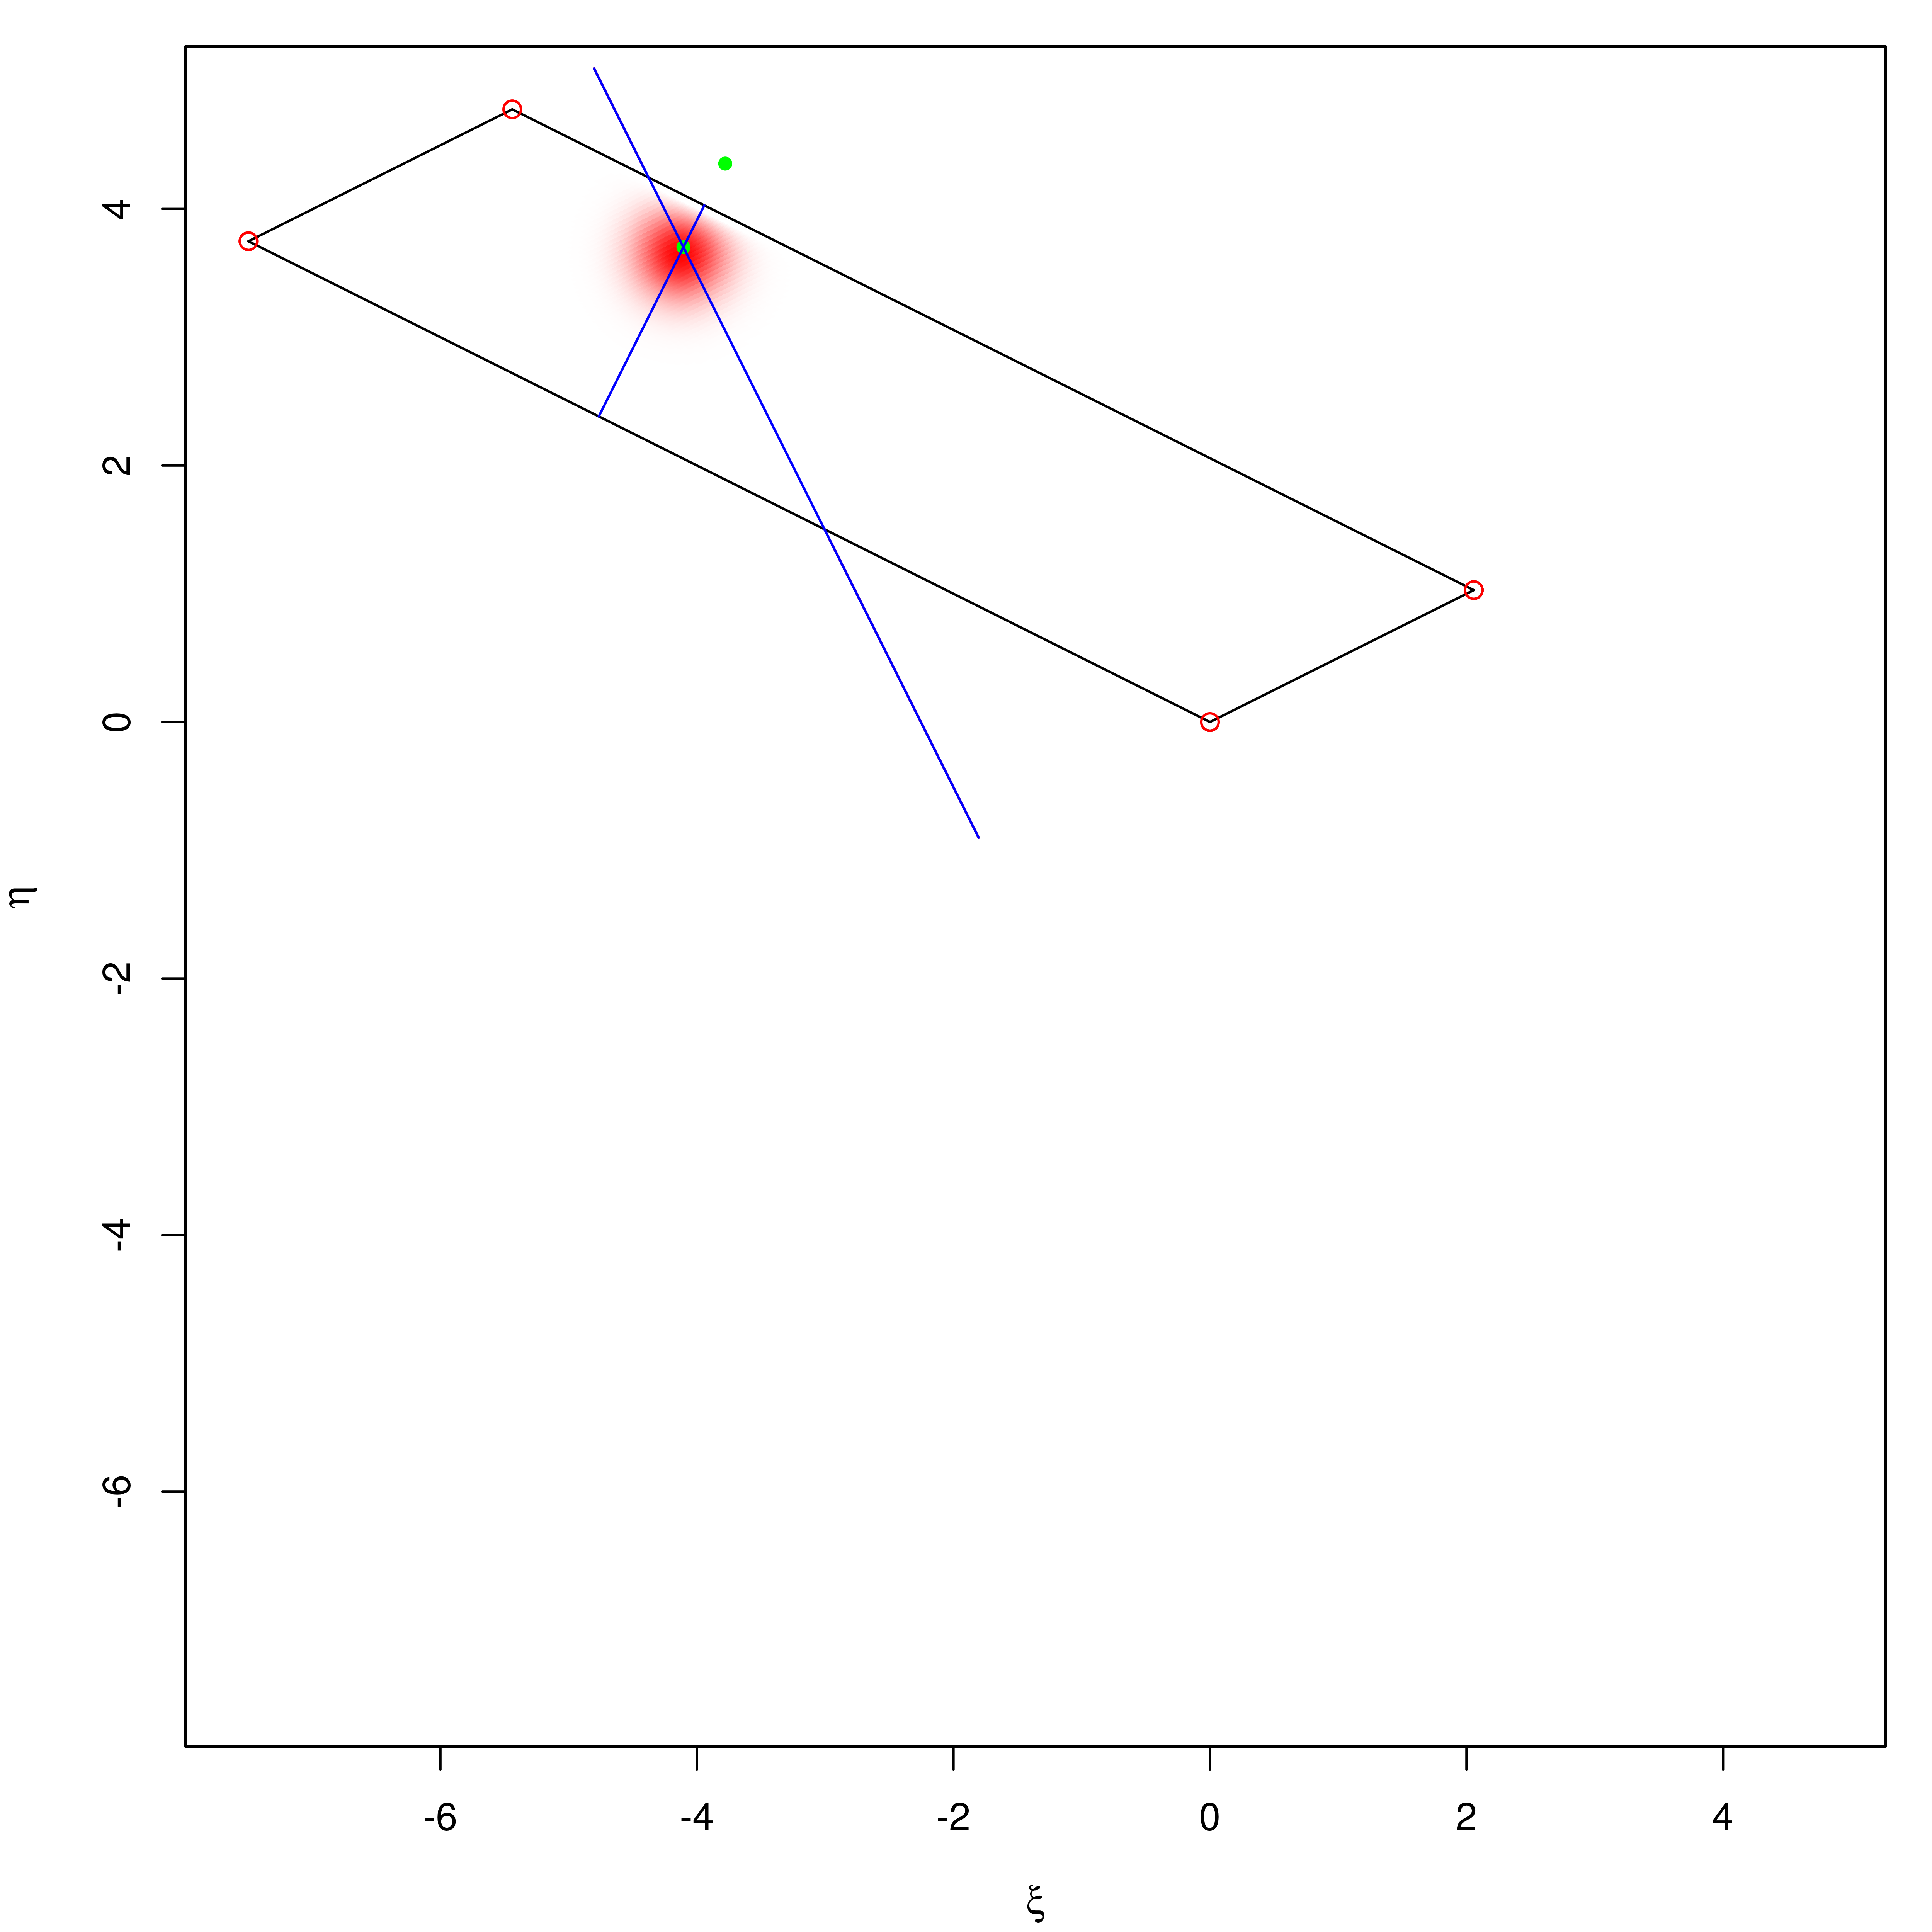
\includegraphics[width=1\linewidth]{../small-time-solution.png}
    \end{minipage}p
    %%
    & \begin{minipage}{0.5\textwidth}
      \centering
      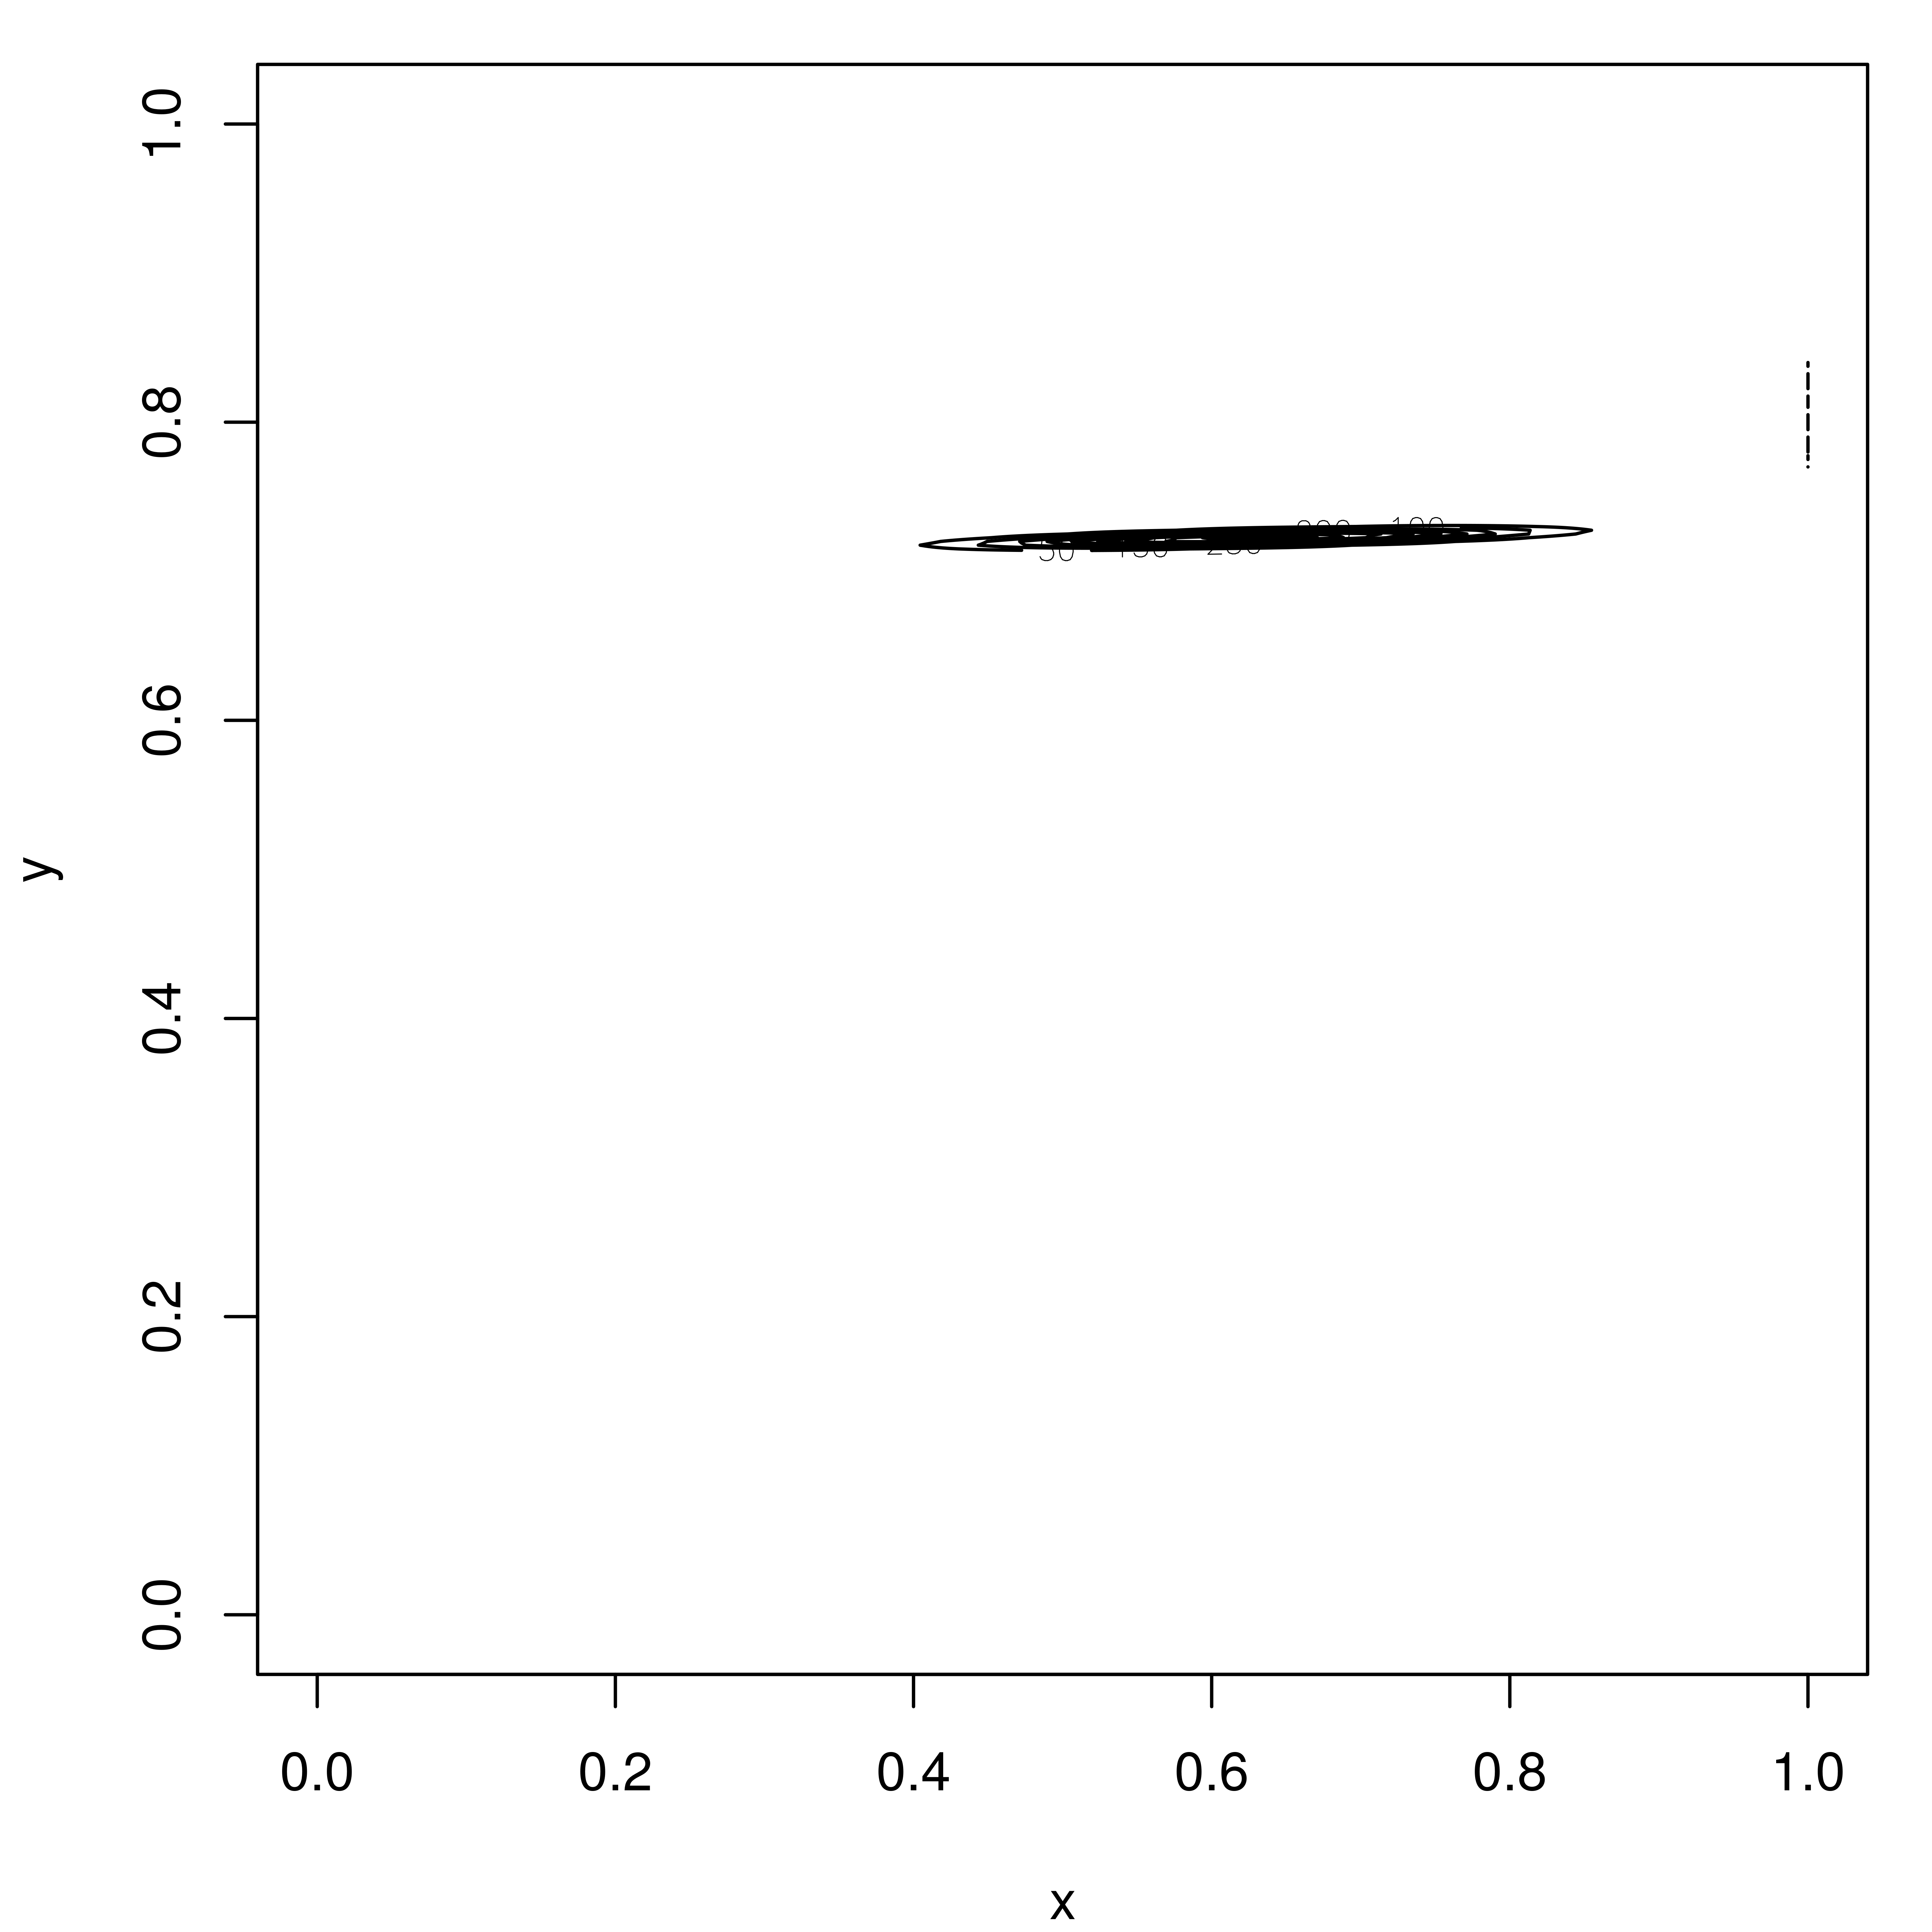
\includegraphics[width=1\linewidth]{../small-time-solution-contour.png}
    \end{minipage}
  \end{tabular}
  %%
  %%
  \caption{An example of the small-time solution
    $p(\xi,\eta,t_\epsilon)$ on the transformed domain
    $\tilde{\Omega}$ with $\tau_x = \tau_y = 1$ and $\rho=0.6$. Right:
    The shaded red region is a heatmap of the small-time solution in
    the transformed coordinate frame, while the blue line segments
    represent the distance between the boundaries and the initial
    condition coordinate. The green point outside of the computational
    domain is the center of the reflected image $(\xi_0', \eta_0')$
    about the closest boundary. Left: The small-time solution
    transformed back to the original coordinate system. Here, the
    contours denote the level-sets for the function. They very closely
    approximate the level sets for the fundamental solution of the
    unbounded problem (\ref{eq:qq})}
  \label{fig:step-1-small-time}
\end{figure}
Using Theorem 5.E of \cite{zeidler1995applied}, we can solve for
$p(\tilde{x},\tilde{y},\tilde{t})$ by considering the smooth
$p(\tilde{x},\tilde{y},\tilde{t}_\epsilon)$ as an initial condition
and evolving it forward in time by $\tilde{t} -
\tilde{t}_\epsilon$. This replaces initial condition in
(\ref{eq:orthogonality-conditions-mat-2}) with
\begin{align}
  M \mathbf{c}(\tilde{t}_\epsilon) &= \mathbf{p}(\tilde{t}_\epsilon), \\
  [\mathbf{p}(\tilde{t}_\epsilon)]_i &= \displaystyle \int_{\tilde{\Omega}} p(\tilde{x},\tilde{y},\tilde{t}_\epsilon) \psi_i(\tilde{x},\tilde{y}) d\tilde{x}\,d\tilde{y}. \nonumber
\end{align}
Intuitively, the bigger $\tilde{t}_\epsilon$, the smaller both
$R_e(k)$ and $R_0(k)$ will be in approximating the solution for the
initial value $p(\tilde{x},\tilde{y},\tilde{t}_\epsilon)$. On the
other hand, for large $\tilde{t}_\epsilon$, the error in the
small-time approximate solution will be significant. The selection of
$\tilde{t}_\epsilon = d_2/8$ is a good compromise for accommodating
these two opposing forces in reducing errors.
% less eigenmodes present in $p(\tilde{x},\tilde{y},\tilde{t}_\epsilon)$, and the more accurate
% our weak solution according to the error estimate
% \[
%   \| e(t) \|_{L_2(\Omega)} \leq C h(k)^2 \| p(\tilde{x},\tilde{y},\tilde{t}_\epsilon) \|_{2}.
% \]


\subsection{Basis Family} \label{sec:basis-family}
% An upper bound of the rate at which the Galerkin approximation
% converges to $p(\tilde{x},\tilde{y},\tilde{t})$ is given by condition (\ref{eq:ic-bound}),
% namely by how well the initial condition may be approximated via a
% projection onto $S_k$.
We motivate the construction of the basis functions by
once again considering the fundamental solution for the unbounded
problem (\ref{eq:qqq}). We choose the family of basis functions
$S_k = \left\{\psi_i(\tilde{x},\tilde{y}), \,\, 0 \leq i \leq k \right\}$
\begin{align}
  \psi_i(\tilde{x},\tilde{y}) &= \frac{1}{2\pi \tilde{\sigma}^2\sqrt{1-\tilde{\rho}^2} } \\
                              &\quad \times \exp\left\{ -\frac{\left( (\tilde{x} - \tilde{x}_i)^2 - 2\tilde{\rho} (\tilde{x}-\tilde{x}_i)(\tilde{y}-\tilde{y}_i) + (\tilde{y} - \tilde{y}_i)^2 \right)}{2(1-\tilde{\rho}^2)\tilde{\sigma}^2}  \right\} \nonumber \\
  &\quad \times \tilde{x}\left(1-\tilde{x}\right)\, \tilde{y}(1-\tilde{y}) \nonumber
\end{align}
for some parameters $(\tilde{\rho}, \tilde{\sigma})$ and a collection of nodes
$\{ (\tilde{x}_i,\tilde{y}_i) \}_{i=0}^k$ which form a grid over
$\tilde{\Omega}$.

This grid is determined by the choice of kernel parameters
$(\tilde{\rho}, \tilde{\sigma})$ with a scaling parameter $l$, and it
is defined in the following way. For a set of
$(\tilde{\rho}, \tilde{\sigma}, l)$, shift the coordinate system so
that $(\tilde{x}_0', \tilde{y}_0') = (1/2,1/2)$. In the shifted
coordinate system, generate a rectangular grid, uniform in each of
$x$- and $y$-directions, over the square region
$[1/2 - 1/\sqrt{2}, 1/2+1/\sqrt{2}] \times [1/2 - 1/\sqrt{2},
1/2+1/\sqrt{2}]$. The grid size in the $x$-direction is set to
$l\tilde{\sigma}(1+\tilde{\rho})$ and the grid size in the
$y$-direction is $l\tilde{\sigma}(1-\tilde{\rho})$. The square region
is selected to ensure that after a $\pi/4$ rotation around
$(1/2, 1/2)$, the rotated grid should cover the square
$[0, 1] \times [0, 1]$ (see left panel of Figure (\ref{fig:grids})).

%%
%%
\begin{figure}
  \centering
  %%
  %%
  \begin{tabular}{cc}
    \begin{minipage}{0.4\textwidth}
      \centering
      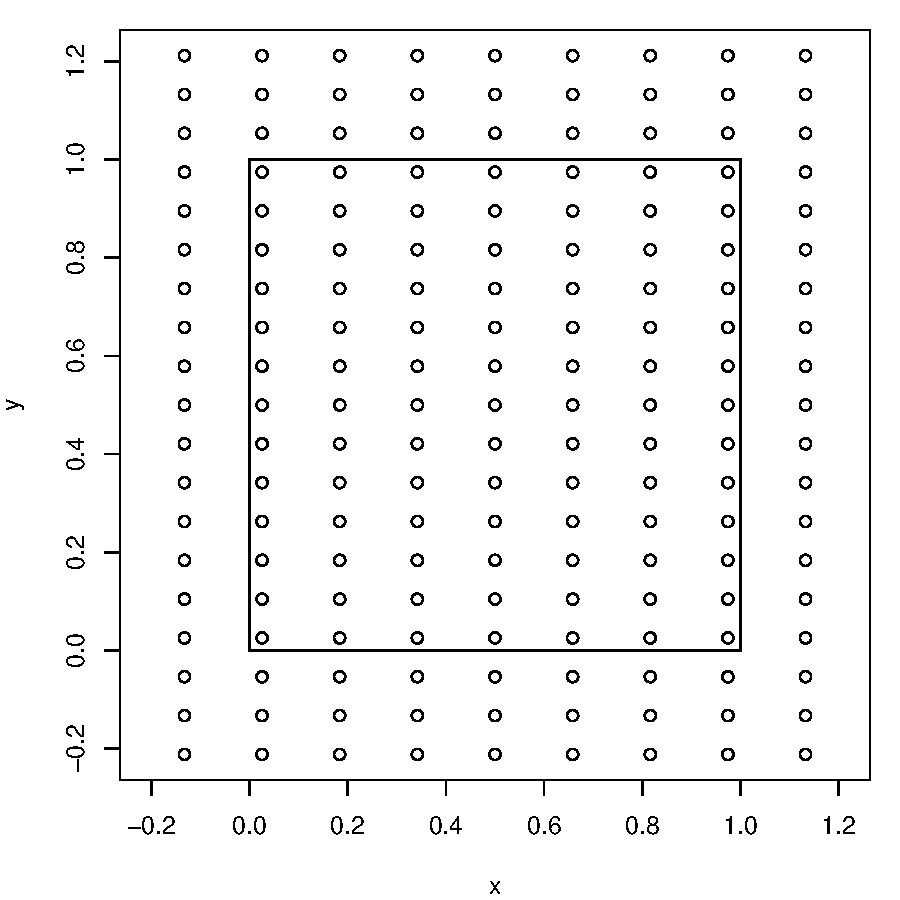
\includegraphics[width=1\linewidth]{../nodes-1.pdf}
    \end{minipage}
    %%
    & \begin{minipage}{0.4\textwidth}
      \centering
      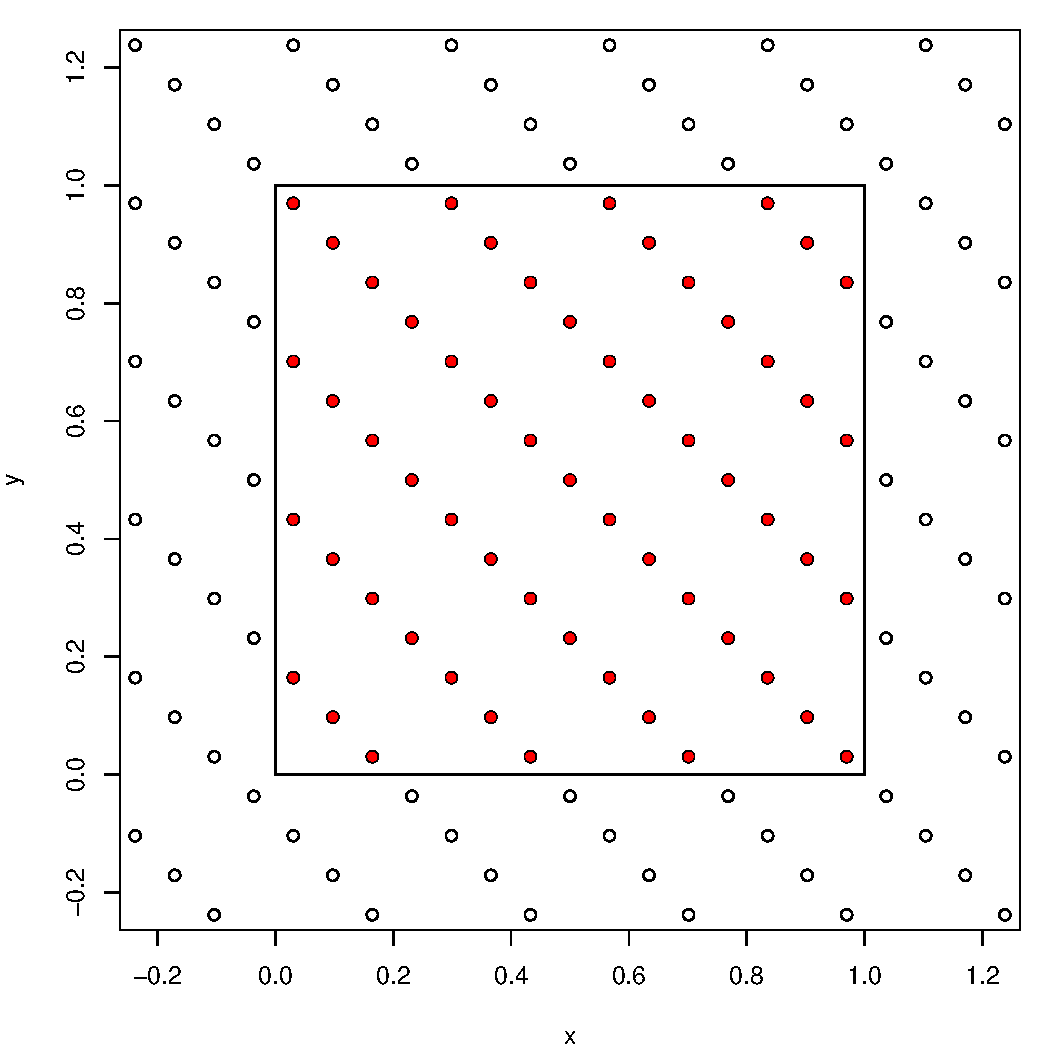
\includegraphics[width=1\linewidth]{../nodes-2.pdf}
    \end{minipage}
  \end{tabular}
  %%
  %%
  \caption{A sample grid design for $l=1$, $\sigma=0.3$ and $\rho=0.6$. The
    left panel corresponds to the initial grid
    $\{ (x'_j,y'_j) \}_{j=0}^{k'}$ over $\Omega$ (solid black
    square). The right panel depicts the rotated initial grid. The set
    of final node points $\{ (x_i,y_i) \}_{i=0}^{k}$ is contained
    within $\Omega$ and is denoted by the red solid points.}
  \label{fig:grids}
\end{figure}
%%
%%
% Next, apply the clockwise, $\pi/4$ rotation centered on
% $(1/2, 1/2)$ to each node
% \begin{align*}
%   \left( \begin{array}{c}
%            \tilde{x}_j \\
%            \tilde{y}_j
%          \end{array} \right) =
%        \left( \begin{array}{cc}
%                 1/\sqrt{2} & 1/\sqrt{2} \\
%                 -1/\sqrt{2} & 1/\sqrt{2}
%               \end{array} \right)
%             \left( \begin{array}{c}
%                      \tilde{x}'_j - 1/2\\
%                      \tilde{y}'_j -1/2
%                    \end{array} \right) +
%   \left( \begin{array}{c}
%            1/2 \\ 1/2
%            \end{array} \right).
% \end{align*}
The grid is comprised of all nodes within $\tilde{\Omega}$:
\[\left\{(\tilde{x}_i, \tilde{y}_i)\right\}_{i=0}^k = \left\{
    (\tilde{x}_j, \tilde{y}_j) | (\tilde{x}_j, \tilde{y}_j) \in
    \tilde{\Omega}, j = 0, \ldots, k' \right\}, \] (see right panel of
Figure (\ref{fig:grids})). It should be noted that the level sets of
the heat kernel for the basis functions are ellipses with major and
minor axes aligned with the node points. Further, there is more
resolution (ie. the node layout is denser) along the direction
corresponding to the smaller standard deviation of the basis heat
kernel in the principal coordinate frame. Finally, for a given $l$,
nodes in either principal direction are separated by $l$ standard
deviations of the basis heat kernel. This layout naturally takes into
account some degree of correlation $\tilde{\rho}$ so that the
small-time solution, having level sets similar to those of the
kernels, can be better resolved. Essentially, the collection
$\{ \psi_i(\tilde{x},\tilde{y}| \tilde{\rho}, \sigma) \}_{i=0}^k$ is
composed of fundamental solutions to a heat diffusion problem tuned by
$\sigma$ and $\tilde{\rho}$, tampered such that their support is on
$\tilde{\Omega}$, zero on the boundaries, still smooth, and inheriting
the correlation structure of the fundamental solution to the
problem. For the purposes of this paper, we found that keeping
fixed $l=1$ with a moderate $\tilde{\rho}$ ($|\tilde{\rho}| \sim 0.8$)
yields reasonable results. It is important, however, that
$\mbox{sign}(\tilde{\rho}) = \mbox{sign}(\rho)$ so that the
problematic, narrow component of the small-time solution (which can be
seen in the minor axis of the contours of the small-time solution in
the right panel of Figure (\ref{fig:step-1-small-time})) can be
resolved.
%
%
%In this manner,
% our basis function choice is in keeping with the golden rule for the
% rate of convergence: \textbf{The smoother the solution to the original
%   problem and the smoother the functions in the basis space, the
%   faster the convergence of the Ritz-Galerkin method.} (Remark 1(c) in
%   Chapter 2 of \cite{zeidler1995applied}).
%
% At this point, having explicitly defined
% $\psi_i(\tilde{x},\tilde{y}|\sigma,\tilde{\rho})$, it should be noted that these basis
% functions are constant with respect to the normalized problem
% parameters $(\ \rho)$. Thus, the derivative of Galerkin
% approximation $p^{(k)}$ with respect to the boundaries takes on the
% form
% \[
%   \frac{\partial^4}{\partial a_x \partial b_x \partial a_y \partial
%     b_y} p^{(k)}(x,y,t) = \boldsymbol{\psi}(x,y)^T
%   \frac{\partial^4}{\partial a_x \partial b_x \partial a_y \partial
%     b_y} \left\{ \exp\left( M^{-1}S\, t \right) \mathbf{c}(0) \right\},
% \]
% which is well-defined given the discussion above.

\subsection{Error Bound} \label{sec:error-bound}
A bound on the closeness of the approximate solution $p^{(k)}(\tilde{x},\tilde{y},\tilde{t})$
to the strong solution $p(\tilde{x},\tilde{y},\tilde{t})$ is developed in
\cite{bramble1977some}.  Their result shows that the Galerkin
approximation we use converges to the strong solution in
$L_2(\tilde{\Omega})$, and it motivates the thrust of our numerical
solution. First, we define the \textit{error} term
\[
  e^{(k)}(t) = p(\tilde{x},\tilde{y},\tilde{t}) -
  p^{(k)}(\tilde{x},\tilde{y},\tilde{t}),
\]
as well as the norm
\[
  \| w \|_2 = \sum_{j=0}^\infty \lambda_j^2 \left<w, \phi_j\right>^2
\]
for the eigenpairs $(\lambda_j, \phi_j)$ of the operator
$\mathcal{L}$. The $\| \cdot \|_2$ norm used in \cite{bramble1977some}
captures the variation in a given function: for any set of eigenpairs
$\left\{(\lambda_j, \phi_j)\right\}$ over the domain $\tilde{\Omega}$,
increasing the absolute value of $\lambda_j$ with $j$ corresponds to a
function $\phi_j$ with increasing number of oscillations over
$\tilde{\Omega}$. The $\|\cdot\|_2$ norm is distict from the usual
$L_2(\tilde{\Omega})$ norm , which we denote as
$\|\cdot \|_{L_2(\tilde{\Omega})}$. As referred to in
\cite{bramble1977some}, functions $w \in L_2(\tilde{\Omega})$ with
$\|w\|_2 < \infty$ are also in $W_2^2(\tilde{\Omega})$. Finally, if we
have the condition (corresponding to equation 2.1 in
\cite{bramble1977some})
\begin{align}
  \| p(\tilde{x},\tilde{y},\tilde{t}_\epsilon) - p^{(k)}(\tilde{x},\tilde{y},\tilde{t}_\epsilon) \|_{L_2(\tilde{\Omega})} &\leq C\, h(k)^2 \| p(\tilde{x},\tilde{y},\tilde{t}_\epsilon) \|_2, \label{eq:ic-bound}
\end{align}
where $h(\cdot)$ is a decreasing function of $k > 0$, Theorem 2.1 in
\cite{bramble1977some} applies and we have the error estimate
\begin{align}
  \| e^{(k)}(t) \|_{L_2(\tilde{\Omega})} \leq C h(k)^2 \| p(\tilde{x},\tilde{y},\tilde{t}_\epsilon) \|_{2}. \label{eq:error-est}
\end{align}
Here, the  constant $C$  and the  function $h(k)$ are  the same  as in
(\ref{eq:ic-bound}). The implication is that if the basis functions in
$S_k$ represent  the small-time  solution $p(\tilde{x},\tilde{y},\tilde{t}_\epsilon)$  with no
error, the Galerkin solution forward in time is also without error.

We can ensure condition (\ref{eq:ic-bound}) is met if $S_k$ is
complete in $L_2(\tilde{\Omega})$ as $k$ grows. The other two conditions
necessary for the error bound to apply are demonstrated by
\cite{bramble1977some} for the Galerkin method. Equation
(\ref{eq:error-est}) can be summarized in a simple way: the
\textit{error} of the method is controlled by how much variation the
small-time solution has; the \textit{rate} of decrease of the error is
controlled by how well the span of $S_k$ represents the small-time
solution compared to the variation of the initial condition as $k$
increases. In the context of (\ref{eq:error-est}), our method, with
its small-time analytic solution and choice of basis functions, is
specifically tailored to minimize the error between the strong
solution and its Galerkin approximation under $L_2(\tilde{\Omega})$.

% However, the initial condition for (\ref{eq:qq}) requires all in
% eigenmodes being included in the representation of the initial
% conditions, so that
% \[
%   \| p(x,y,0) \|_{2} = \left\| \delta\left( x - \frac{x_0 - a_x}{b_x-a_x}
%   \right) \delta\left( y - \frac{y_0 - a_y}{b_y-a_y} \right)\right\|_{2} = +\infty.
% \]
% It is obvious that we cannot apply the error estimates above. However,
% evolving the solution forward in time, even for a short period,
% diffuses the delta-function IC and attenuates out the highest
% frequency modes. Further, because solutions to the diffusion equation
% are smooth, $p(x,y,t_\epsilon)$ will give us a smooth initial function
% which will make the error bounds admissible.


\section{Estimation}
The estimation of asset price and volatility is an important problem
in finance. It is common to assume that asset prices follow correlated
geometric Brownian motions.  In that setting, estimates of volatility
and correlation are usually based on daily log-returns, which depend
only on the opening and closing prices.  However, typically more
information is available.  For example, maximum and minimum trading
prices over the days are readily available.  In univariate settings,
it has been shown that incorporating this additional information can
substantially improve estimates.  The pdf from \eqref{eq:pdf} provides
the likelihood necessary for frequentist and Bayesian inference in
bivariate settings.  Likelihood-free approaches, like that of
\cite{rogers1991estimating}, \cite{rogers2008estimating}, on the other
hand suffer from not being able to be easily integrated into
inferential frameworks that require explicit estimates of probability,
as well as being sub-optimal as will be seen in the Simulation section
below.

To illustrate this, we consider maximum
likelihood inference from an i.i.d. sample $Z_1, \ldots, Z_n$, where
$Z_i = (X_i, Y_i, m_{x,i}, M_{x,i}, m_{y,i}, M_{y,i})$, where $X_i$
and $Y_i$ corresponds to log returns of the two assets, $m_{x,i}$ and
$m_{y,i}$ correspond to the minimum log-returns observed during the
day, and $M_{x,i}$ and $M_{y,i}$ correspond to the maximum log
returns.
% Consider the problem of estimating the parameters
% $(\mu_x, \mu_y, \sigma_x, \sigma_y, \rho)$ from an i.i.d. set of
% samples $(Z_1, \ldots, Z_n)$ from random variable $Z(t)$, defined
% below, at a given value of $t$ in the process in
% (1)-(2). Specifically, $Z(t)$ is formed as
% $$ Z(t) =( X(t), Y(t), m_x(t), M_x(t), m_y(t), M_y(t)) $$
% where
% $$m_x(t)= \min_{0 \le t' \le t} X(t), \;\;
% M_x(t)= \max_{0 \le t' \le t} X(t), \;\; m_y(t)= \min_{0 \le t' \le t}
% Y(t), \;\; M_y(t)= \max_{0 \le t' \le t} Y(t). $$ We say that $Z_i$ is
% sampled from the distribution corresponding to the probability density
% function (\ref{eq:pdf})
% \[
%   Z_i \sim F(\theta),
% \]
% where the cumulative distribution function $F$ has the usual interpretation
% \begin{align*}
%   F(z = (x, y, a_x, b_x, a_y, b_y) | \theta) &= \Pr\left(X(t) \leq x,
%     Y(t) \leq y, m_x \leq a_x, M_x \leq b_x, m_y \leq a_y, M_y \leq b_y\right).
% \end{align*}
% This estimation problem is of particular importance in quantitative
% finance where the model equations (\ref{eq:X}) - (\ref{eq:Y}) (with
% various bells and whistles attached) are widely used. However, to the
% best of our knowledge, all current \textit{likelihood} methods in the
% literature either ignore the observed maximum/minimum information or
% use only some of it.
Since we do not have a closed-form solution for the likelihood
\eqref{eq:pdf}, we will use an iterative derivative-free numerical
algorithm to maximize the likleihood which requires repeated
evauluation of the likelihood (the Nelder-Mead method; see
\cite{lagarias1998convergence} for review and convergence
properties). This is feasible even for moderate to large sample sizes,
because our numerical method is specifically designed for
computational efficiency for repeatedly evaluating the density
function (\ref{eq:pdf}). The maximum likelihood estimator (MLE) for
the true parameters based on $n$ samples, which we call
$\hat{\theta}_n := (\hat{\mu}_x, \hat{\mu}_y, \hat{\sigma}_x,
\hat{\sigma}_y, \hat{\rho})$, is especially useful in practical
settings when it exhibits \textit{consistency}, \textit{i.e.}: the MLE
gets closer to the true parameter vector $\theta$ as more data is
collected and included in the likelihood (assuming the model and its
parameters remain constant during the data collection). More
precisely, the estimator $\hat{\theta}_n$ is consistent if it
converges in probability to the true parameter:
\[
  \Pr( | \hat{\theta}_n - \theta | ) \to 0 \qquad \mbox{as} \qquad n \to \infty.
\]

\subsection{Consistency}
In this section we prove that the MLE based on the Galerkin
approximation $p^{(k)}(\tilde{x},\tilde{y},\tilde{t})$ is
consistent. To do so, we first show that the distribution on $Z$ based
on the approximate $p^{(k)}(\tilde{x},\tilde{y},\tilde{t})$ converges
to the true distribution $F(\cdot | \theta)$. Define the approximate probability
density
\begin{align}
  f^{(k)}(x,y,a_x,b_x,a_y,b_y) := \frac{\partial^4}{\partial
  a_x \partial b_x \partial a_y \partial b_y}
  q^{(k)}(\tilde{x},\tilde{y},\tilde{t}). \label{eq:galerkin-density}
\end{align}
At this point we will assume that for a sufficiently large $k$,
$f^{(k)}(z)$ is positivie for all $z \in Z$ and is integrable over
$Z$. As such, we may regard it as a proper probability density
function with the cumulative probability density and probability
measure over $Z$ being
\begin{align}
  F^{(k)}(z | \theta) &= \displaystyle \int_{-\infty}^{a_x} \displaystyle \int_{-\infty}^{a_y} \displaystyle \int_{-\infty}^{b_x} \displaystyle \int_{-\infty}^{b_y} \displaystyle \int_{-\infty}^x \displaystyle \int_{-\infty}^y \frac{\partial^4}{\partial a'_x \partial b'_x \partial a'_y \partial b'_y} q^{(k)}(x', y', t | a'_x, b'_x, a'_y, b'_y)\,\,\, dz, \label{eq:approx-measure} \\
                          \Pr_{k}(A) &:= \displaystyle \int_{A} f^{(k)}(z)\, dz, \quad \mbox{ for any measurable } A \subset Z. \label{eq:approx-measure-2}
\end{align}
We will prove that for every $z \in Z$,
\[
  \lim_{k\to \infty} F^{(k)}(z | \theta) = F(z | \theta).
\]
First, we prove the Lemma
\begin{lemma}\label{lem:1}
  For $z = (x, y, a_x, b_x, a_y, b_y)$,
  \[
    \lim_{k\to \infty} \displaystyle \int_{a_x}^{b_x} \displaystyle
    \int_{a_y}^{b_y} f^{(k)}(x,y,a_x,b_x,a_y,b_y)\, dx\,dy =
    \displaystyle \int_{a_x}^{b_x} \displaystyle \int_{a_y}^{b_y}
    f(x,y,a_x,b_x,a_y,b_y)\, dx\,dy.
  \]
\end{lemma}
\begin{proof}
  Define the sets of form, for $z = (x,y,a_x,b_x,a_y,b_y)$,
  \begin{align*}
    B(a_x, b_x, a_y, b_y) &= \left\{ z' \in Z \left| z' \in [a_x, b_x]
        \times [a_y, b_y] \times [a_x, \infty) \times (-\infty, b_x]
                            \times [a_y, \infty) \times (-\infty, b_y] \right.\right\}.
  \end{align*}
  Elements within $B(a_x, b_x, a_y, b_y)$ are equivalent to sample
  paths that stay within the region $[a_x, b_x] \times [a_y, b_y]$:
  \begin{align*}
    B(a_x, b_x, a_y, b_y) &= \left\{ \omega \in W | X_\omega(t) \in [a_x, b_x], Y_\omega(t) \in [a_y, b_y], m_x \in [a_x,b_x), M_x \in (a_x, b_x] \right\}
  \end{align*}
  Then
  \begin{align}
    \Pr(B(a_x, b_x, a_y, b_y)) &= \displaystyle \int_{B(a_x, b_x, a_y, b_y)} f(z)\, dz \nonumber \\
                               &= \displaystyle \int_{a_y}^{\infty} \displaystyle \int_{-\infty}^{b_y} \displaystyle \int_{a_x}^{\infty} \displaystyle \int_{-\infty}^{b_x} \displaystyle \int_{-\infty}^{b_x} \displaystyle \int_{-\infty}^{b_y} f(x', y', a'_x, b'_x, a'_y, b'_y) dx' dy' da_x' db_x' da_y' db_y' \label{eq:full-form} \\
                               &= \displaystyle \int_{a_x}^{b_x} \displaystyle \int_{a_y}^{b_y} q(x,y,a_x,b_x,a_y,b_y)\, dx\, dy, \nonumber
  \end{align}
  where the last equality employs the interpretation of $q$ in
  (\ref{eq:CDF}) and we can freely change the order of integration as
  $f$ is bounded for all $z \in Z$. Similarly,
  \begin{align*}
    \Pr_k(B(a_x, b_x, a_y, b_y)) &= \displaystyle \int_{a_x}^{b_x} \displaystyle \int_{a_y}^{b_y} q^{(k)}(x,y,a_x,b_x,a_y,b_y)\, dx\, dy.
  \end{align*}
  From (\ref{eq:full-form}), the partial derivative of the probability
  $\Pr(B(a_x,b_x,a_y,b_y))$ is well-defined and can be written as
  \begin{align*}
    \frac{\partial^4}{\partial a_x \partial b_x \partial a_y \partial b_y} \Pr(B(a_x, b_x, a_y, b_y)) &= \displaystyle \int_{a_x}^{b_x} \displaystyle \int_{a_y}^{b_y} f(x,y,a_x,b_x,a_y,b_y)\, dx\, dy.
  \end{align*}
  The second-order \textbf{finite difference} approximation the above
  expression can be expressed as a linear combination of probabilities
  of perturbed sets $B(\cdot)$:
  \begin{align*}
    \lim_{\epsilon \to 0}\quad \frac{1}{\epsilon^4} \sum_{i=1}^{16} c(i) \Pr(B(a_x + k_1(i)\epsilon, b_x + k_2(i)\epsilon, a_y + k_3(i)\epsilon, b_y + k_4(i)\epsilon) &= \\
    \MoveEqLeft[8] \frac{\partial^4}{\partial a_x \partial b_x \partial a_y \partial b_y} \Pr(B(a_x, b_x, a_y, b_y)),
  \end{align*}
where $c(i)$ and $k(i)$ are functions mapping index $i$ to the
corresponding coefficient in the second-order finite difference
approximation
  $c(i) \to \left\{-1, 1\right\}$, $k_j(i) \to \{-1,1\}$. Using Big-O
  notation, for a sufficiently small $\epsilon$
  \begin{align}
    \sum_{i=1}^{16} c(i) \Pr(B(a_x + k_1(i)\epsilon, b_x +
    k_2(i)\epsilon, a_y + k_3(i)\epsilon, b_y + k_4(i)\epsilon) &= \nonumber \\
    \MoveEqLeft[10] \epsilon^4 \frac{\partial^4}{\partial a_x \partial b_x \partial
      a_y \partial b_y} \Pr(B(a_x, b_x, a_y, b_y)) + O(\epsilon^6 ;
    a_x, b_x, a_y, b_y). \label{eq:fin-diff}
  \end{align}
  The convergence result in Section \ref{sec:error-bound} implies that
  \begin{align*}
    \Pr_k(B(a_x + k_1(i)\epsilon, b_x + k_2(i)\epsilon, a_y +
    k_3(i)\epsilon, b_y + k_4(i)\epsilon) &= \\
    \MoveEqLeft[10] \displaystyle \int_{a_x +
    k_1(i)\epsilon}^{b_x + k_2(i)\epsilon} \displaystyle \int_{a_y + k_3(i)\epsilon}^{b_y +
    k_4(i)\epsilon} q^{(k)}(x,y,a_x,b_x,a_y,b_y)\, dx\, dy \to \\
   \displaystyle
     \int_{a_x + k_1(i)\epsilon}^{b_x + k_2(i)\epsilon} \displaystyle \int_{a_y +
     k_3(i)\epsilon}^{b_y + k_4(i)\epsilon} q(x,y,a_x,b_x,a_y,b_y)\, dx\, dy &= \\
    \MoveEqLeft[20] \Pr(B(a_x + k_1(i)\epsilon, b_x + k_2(i)\epsilon, a_y +
    k_3(i)\epsilon, b_y + k_4(i)\epsilon) \mbox{ as } k \to \infty \mbox{ in } L_2(\Omega).
  \end{align*}
  Hence, for a sufficiently large $k$ dependent on the supremum over
  $i$, and given the error estimate in (\ref{eq:error-est}), we obtain
  the relation
  \begin{align*}
    \Pr_k(B(a_x + k_1(i)\epsilon, b_x + k_2(i)\epsilon, a_y +
    k_3(i)\epsilon, b_y + k_4(i)\epsilon) &= \\
    \Pr(B(a_x + k_1(i)\epsilon, b_x + k_2(i)\epsilon, a_y +
    k_3(i)\epsilon, b_y + k_4(i)\epsilon) &\\
    + O(h(k)^2; a_x + k_1(i)\epsilon, b_x + k_2(i)\epsilon, a_y + k_3(i)\epsilon, b_y + k_4(i)\epsilon) &
  \end{align*}
  Note here that the dominating terms $O(h(k)^2; \cdot)$ are
  differentiable with respect to the boundary parameters
  $(a_x, b_x, a_y, b_y)$ since $q$ and $q^{(k)}$ have this
  property. Therefore, if we replace $\Pr(\cdot)$ in
  (\ref{eq:fin-diff}) with $\Pr_k(\cdot)$
  \begin{align*}
    \sum_{i=1}^{16} c(i) \Pr_k(B(a_x + k_1(i)\epsilon, b_x +
    k_2(i)\epsilon, a_y + k_3(i)\epsilon, b_y + k_4(i)\epsilon) &= \\
    \sum_{i=1}^{16} c(i) \Pr(B(a_x + k_1(i)\epsilon, b_x +
    k_2(i)\epsilon, a_y + k_3(i)\epsilon, b_y + k_4(i)\epsilon) &  \\
    + \sum_{i=1}^{16} c(i) O(h(k)^2; a_x + k_1(i)\epsilon, b_x +
    k_2(i)\epsilon, a_y + k_3(i)\epsilon, b_y + k_4(i)\epsilon) &= \\
    \epsilon^4 \frac{\partial^4}{\partial a_x \partial b_x \partial
    a_y \partial b_y} \Pr(B(a_x, b_x, a_y, b_y)) + O(\epsilon^6 ;
    a_x, b_x, a_y, b_y) & \\
    + \sum_{i=1}^{16} c(i) O(h(k)^2; a_x + k_1(i)\epsilon, b_x +
    k_2(i)\epsilon, a_y + k_3(i)\epsilon, b_y + k_4(i)\epsilon). &
  \end{align*}
  Dividing both sides by $\epsilon^4$ produces
  \begin{align*}
    \frac{1}{\epsilon^4} \sum_{i=1}^{16} c(i) \Pr_k(B(a_x + k_1(i)\epsilon, b_x +
    k_2(i)\epsilon, a_y + k_3(i)\epsilon, b_y + k_4(i)\epsilon) &= \\
    \frac{\partial^4}{\partial a_x \partial b_x \partial
    a_y \partial b_y} \Pr(B(a_x, b_x, a_y, b_y)) + O(\epsilon^2;
    a_x, b_x, a_y, b_y) \\
    + \frac{1}{\epsilon^4}\sum_{i=1}^{16} c(i) O(h(k)^2; a_x + k_1(i)\epsilon, b_x +
    k_2(i)\epsilon, a_y + k_3(i)\epsilon, b_y + k_4(i)\epsilon).
    % = \frac{\partial^4}{\partial a_x \partial b_x \partial
    % a_y \partial b_y} \Pr(B(a_x, b_x, a_y, b_y)) + O(\epsilon;
    % a_x, b_x, a_y, b_y) + \frac{\partial^4}{\partial a_x \partial b_x \partial
    % a_y \partial b_y} O(h(k)^2 ; a_x, b_x, a_y, b_y)
  \end{align*}
  As mentioned above $O(h(k)^2; \cdot)$ is differentiable with respect
  to the boundary parameters, so that the right-most term is still
  $O(h(k)^2)$ as $\epsilon \to 0$. Taking the limit in $\epsilon$, we have
  \begin{align*}
    \displaystyle \int_{a_x}^{b_x} \displaystyle \int_{a_y}^{b_y}
    f^{(k)}(x,y,a_x,b_x,a_y,b_y)\, dx\, dy =
    \frac{\partial^4}{\partial a_x \partial b_x \partial a_y \partial
    b_y} \Pr_k(B(a_x, b_x, a_y, b_y)) \\
    = \frac{\partial^4}{\partial
      a_x \partial b_x \partial a_y \partial b_y} \Pr(B(a_x, b_x, a_y,
    b_y)) +  O(h(k)^2; a_x, b_x, a_y, b_y) \\
    =\displaystyle \int_{a_x}^{b_x} \displaystyle \int_{a_y}^{b_y}
    f(x,y,a_x,b_x,a_y,b_y)\, dx\, dy + O(h(k)^2; a_x, b_x, a_y, b_y).
  \end{align*}
  Therefore, we have the desired result:
  \[
    \lim_{k\to \infty} \displaystyle \int_{a_x}^{b_x} \displaystyle
    \int_{a_y}^{b_y} f^{(k)}(x,y,a_x,b_x,a_y,b_y)\, dx\,dy =
    \displaystyle \int_{a_x}^{b_x} \displaystyle \int_{a_y}^{b_y}
    f(x,y,a_x,b_x,a_y,b_y)\, dx\,dy.
  \]
\end{proof}

\begin{lemma}[Convergence in distribution] \label{lem:conv-dist}
  For any $z \in Z$,
  $ \lim_{k \to \infty} F^{(k)}(z | \theta) = F(z).$

\end{lemma}

\begin{proof}
  Let
  \[
    I^{(k)}(z) = \displaystyle \int_{a_x}^{x} \displaystyle
    \int_{a_y}^{y} f^{(k)}(u,v,a_x,b_x,a_y,b_y)\, du\,dv
  \]
  and let
  \[
    I(z) = \displaystyle \int_{a_x}^{x} \displaystyle \int_{a_y}^{y}
    f(u,v,a_x,b_x,a_y,b_y)\, du\,dv.
  \]
  It is possible to show that $\lim_{k\to \infty} I^{(k)}(z) = I(z)$
  as a consequence of Lemma \ref{lem:1} by considering some
  $\chi_k(z) \in S_k$ approximating the indicator
  $1(u \leq x, v \leq y)$ as $k \to \infty$ and setting up a triangle
  inequality. However, we will omit this technical detail here.

  Next, we know that $I(z)$ is integrable over $(a_x, b_x, a_y, b_y)$
  as $\Pr(Z) = \mathbb{P}_{W}(W) = 1$. The Dominated Convergence
  Theorem applies, and we therefore have
  \[
    \lim_{k \to \infty} \displaystyle \int_{-\infty}^{a_x} \displaystyle \int_{-\infty}^{b_x} \displaystyle \int_{-\infty}^{a_y} \displaystyle \int_{-\infty}^{b_y} I^{(k)}(z) da_x' db_x' da_y' db_y' = \displaystyle \int_{-\infty}^{a_x} \displaystyle \int_{-\infty}^{b_x} \displaystyle \int_{-\infty}^{a_y} \displaystyle \int_{-\infty}^{b_y} I(z) da_x' db_x' da_y' db_y',
  \]
  which implies the result of the Lemma.
\end{proof}
% \begin{align*}
%   q(x,y,t) = \\
%   \Pr\left(X(t) \in dx, Y(t) \in dy,  \min_{t'}X(t') \geq a_x,
%   \max_{t'}X(t')\leq b_x, \min_{t'} Y(t')\geq a_y, \max_{t'} Y(t')\leq b_y|  X(0)=x_0, Y(0)=y_0, \theta \right) = \\
%   \Pr_{W}\left(\left\{ \omega \in \Omega | X_\omega(t) \in dx,\,\, Y_\omega(t) \in dy,\,\,  \forall t' \in [0,t]\,\, a_x \leq X_\omega(t') \leq b_x,\,\, \forall t' \in [0,t] \,\, a_b \leq Y_\omega(t') \leq b_y,\,\, X_\omega(0) = Y_\omega(0) = 0 \right\} \right)
% \end{align*}
% Our strategy will be to define a family of sets $\left\{ \tilde{A}_m(z) \right\}_{m=0}^\infty$ for any $z=(x,y,a_x,b_x,a_y,b_y)$ such that
% \begin{align*}
%   \lim_{m \to \infty} \Pr_W \left(  \tilde{A}_m(z) \right) =
%   \Pr \left( X(t) \leq x,
%   Y(t) \leq y, \min_{t' \leq t} X(t') \leq a_x, \max_{t' \leq t}
%   X(t') \leq b_x, \min_{t' \leq t} Y(t') \leq a_y, \max_{t' \leq t}
%   Y(t') \leq b_y \right) = F(z | \theta)
% \end{align*}

% \begin{lemma}
%   For $z = (x,y,a_x,b_x,a_y,b_y)$,
%   \[\lim_{m \to \infty} \displaystyle \int_{-\infty}^x \displaystyle
%     \int_{-\infty}^y q(x',y',t, a_x-m, b_x, a_y-m, b_y)\,\, dx'\,dy' -
%     \displaystyle \int_{-\infty}^x \displaystyle \int_{-\infty}^y
%     q(x',y',t, a_x, b_x, a_y, b_y)\,\, dx'\,dy' = F(z | \theta)\]
% \end{lemma}
% \begin{proof}
% Given some $z = (x,y,a_x,b_x,a_y,b_y)$, define the sets
% \begin{align*}
%   A_m(z) &= \left\{ \omega \in \Omega | X_\omega(t) \leq x,\,\,
% Y_\omega(t) \leq y,\,\, \right. \\ & \forall t' \in [0,t]\,\, a_x-m
% \leq X_\omega(t') \leq b_x,\,\, \\ & \forall t' \in [0,t] \,\, a_y -
% m\leq Y_\omega(t') \leq b_y,\,\, \\ & \left.X_\omega(0) = Y_\omega(0)
% = 0 \right\}, \quad \quad m = 0,1,2,... \\
% \end{align*}
% Note here that $\Pr_{W}(A_m(z)) = \displaystyle \int_{-\infty}^x \displaystyle \int_{-\infty}^y q(x',y',t, a_x-m, b_x, a_y-m, b_y)\,\, dx'\,dy'$.  Next, we define
% \begin{align*}
%   \tilde{A}_{m}(z) &= A_m(z) \,\, \bigcap \,\, A_0^C(z) \\
%                    &= \left\{ \omega \in \Omega | X_\omega(t) \in dx,\,\, \right.\\
%                    & \quad \quad \forall t' \in [0,t]\,\, a_x-m \leq X_\omega(t') \leq b_x,\,\, \\
%                    & \quad \quad \forall t' \in [0,t] \,\, a_y - m\leq Y_\omega(t') \leq b_y,\,\, \\
%                    & \quad \quad \exists t_{a_x} \in [0,t] \,\, s.t. \,\, X_\omega(t_{a_x}) < a_x \,\, , \exists t_{a_y} \in [0,t] \,\, s.t. \,\, X_\omega(t_{a_y}) < a_y, \\
%                    & \quad \quad \left.X_\omega(0) = Y_\omega(0) = 0 \right\}
% \end{align*}
% It is easy to see that $A_{m}(z) \subset A_{m+1}(z)$ and that
% $\tilde{A}_{m}(z) \subset \tilde{A}_{m+1}(z)$. Because of the former
% relation,
% \[
%   \Pr_{W}(\tilde{A}_m(z)) = \Pr_W(A_m(z)) - \Pr_{W}(A_0(z)) = \displaystyle \int_{-\infty}^x \displaystyle \int_{-\infty}^y q(x',y',t, a_x-m, b_x, a_y-m, b_y)\,\, dx'\,dy' - \displaystyle \int_{-\infty}^x \displaystyle \int_{-\infty}^y q(x',y',t, a_x, b_x, a_y, b_y)\,\, dx'\,dy'.
% \]
% Finally,
% \begin{align*}
%   \bigcup_{m=0}^\infty \tilde{A}_m(z) &= \left\{ \omega \in \Omega | X_\omega(t) \in dx,\,\, \right.\\
%                    & \quad \quad \forall t' \in [0,t]\,\, -\infty \leq X_\omega(t') \leq b_x,\,\, \\
%                    & \quad \quad \forall t' \in [0,t] \,\, -\infty \leq Y_\omega(t') \leq b_y,\,\, \\
%                    & \quad \quad \exists t_{a_x} \in [0,t] \,\, s.t. \,\, X_\omega(t_{a_x}) < a_x \,\, , \exists t_{a_y} \in [0,t] \,\, s.t. \,\, X_\omega(t_{a_y}) < a_y, \\
%                    & \quad \quad \left.X_\omega(0) = Y_\omega(0) = 0 \right\},
% \end{align*}
% such that for $\omega \in \bigcup_{m=0}^\infty \tilde{A}_m(z)$,
% $X_\omega(t) \leq x, Y_\omega(t) \leq y, \min_{t'} X_{\omega}(t') \leq
% a_x, \min_{t'} Y_{\omega}(t') \leq a_y, \max_{t'} X_{\omega}(t') \leq
% b_x$, $\max_{t'} Y_{\omega}(t') \leq b_y$, and
% \[
%   \Pr_W\left( \bigcup_{m=0}^\infty \tilde{A}_m(z) \right) = \lim_{M \to \infty} \Pr_W\left( \bigcup_{m=0}^M \tilde{A}_M(z) \right) = F(z |
%   \theta).
% \]
% Since $\tilde{A}_{m}(z) \subset \tilde{A}_{m+1}(z)$,
% \[
%   \lim_{m\to \infty} \Pr_W(\tilde{A}_m(z)) = \lim_{m \to \infty} \displaystyle \int_{-\infty}^x \displaystyle \int_{-\infty}^y q(x',y',t, a_x-m, b_x, a_y-m, b_y)\,\, dx'\,dy' - \displaystyle \int_{-\infty}^x \displaystyle \int_{-\infty}^y q(x',y',t, a_x, b_x, a_y, b_y)\,\, dx'\,dy'  = F(z | \theta)
% \]
% \end{proof}
% For a shorthand, denote
% $
%   \mu_k(\tilde{A}_m(z)) = \displaystyle \int_{-\infty}^x \displaystyle \int_{-\infty}^y q_k(x',y',t, a_x-m, b_x, a_y-m, b_y)\,\, dx'\,dy' - \displaystyle \int_{-\infty}^x \displaystyle \int_{-\infty}^y q_k(x',y',t, a_x, b_x, a_y, b_y)\,\, dx'\,dy'.
% $

% \begin{lemma} \label{lem:weak}
%   For a fixed $m$, $\mu_k(\tilde{A}_m(z)) \to \Pr_W(\tilde{A}_m(z))$ as $k\to \infty$.
% \end{lemma}
% \begin{proof}
%   The proof for this lemma follows direcly from the convergence result
%   $p^{(k)} \to p$ as $k\to \infty$ under the $L_2(\Omega)$ norm from
%   Section \ref{sec:semidiscrete-galerkin}.
% \end{proof}
% With the result from Lemma \ref{lem:weak}, we can now define the
% function $k(m; z)$ as
% \[
%   k(m; z) := \inf_{k'}\left\{ \left| \mu_{k'}(\tilde{A}_m(z)) - \Pr_W(\tilde{A}_m(z)) \right| < 1/2m  \right\}
% \]

% \begin{lemma}\label{lem:convergence-in-dist}
%   For $F_{k(m;z)}$, $F$, and $z$ defined above,
%   \[ \lim_{m\to \infty} F_{k(m;z)}(z | \theta) = F(z | \theta). \]
% \end{lemma}

% \begin{proof}
%   For any $\epsilon > 0$, let $M_1 = 2/\epsilon$. By Lemma
%   \ref{lem:1}, we can find $M_2$ such that $\forall m > M_2$
%   $\left| \Pr_W(\tilde{A}_m(z) - F(z | \theta) \right| <
%   \epsilon/2$. Let $M = \max\{M_1, M_2\}$. For any $m > M$,
%   \begin{align*}
%     \left| F_{k(m)}(z) - F(z) \right | &= \left| \mu_{k(m)}(\tilde{A}_m(z)) - F(z) \right | \\
%                                        &\leq \left|  \mu_{k(m)}(\tilde{A}_m(z)) - \Pr_W(\tilde{A}_m(z)) \right| + \left|  \Pr_W(\tilde{A}_m(z)) - F(z | \theta) \right|. \\
%                                        &\leq \epsilon/2 + \epsilon/2
%   \end{align*}
%   The left term bound is defined by $k(m;z)$.
% \end{proof}

% % \begin{lemma}
% %   For a fixed $k$,
% %   $\lim_{m\to \infty} \mu_k(\tilde{A}_m(z)) = c \in \mathbb{R},$ i.e.
% %   $\left\{ \mu_k(\tilde{A}_m(z))\right\}_{m=0}^\infty$ is a convergent
% %   sequence.
% % \end{lemma}

% % \begin{proof}[Proof idea]
% %   Here we will present a formal argument, without giving all of the
% %   necessary technical details. As $m \to \infty$, the parameters
% %   $\tau_x, \tau_y$ in the normalized problem are $O(1/m)$.  Further,
% %   the initial condition coordinates tend to
% %   $((1-1/m),(1-1/m))$. Letting $\gamma = 1/m$ for $m >> 1$, the
% %   normalized problem becomes
% %   \begin{equation*}
% %     \frac{\partial}{\partial t} p(x,y,t) = \mathcal{L}p(x,y,t),\quad (x,y) \in = \Omega
% % \end{equation*}
% % with the initial condition
% % \begin{align*}
% %   p(x,y,0) &= \delta\left( x - (1-\gamma) \right) \delta\left(y-(1-\gamma)\right),
% % \end{align*}
% % where the differential operator $\mathcal{L}$ is of order
% % \[
% %   \mathcal{L} = \frac{1}{2} \gamma^2 \frac{\partial^2}{\partial x^2}
% %   + \rho\gamma^2 \frac{\partial^2}{\partial x \partial y} + \frac{1}{2}\gamma^2 \frac{\partial^2}{\partial y^2}.
% % \]
% % This means that fundamental solution to the unbounded problem above is
% % the Gaussian density
% % \[
% %   G(x,y,t'| \gamma) = \frac{1}{2\pi\,\,t'\,\, \gamma^2\sqrt{1-\rho^2}} \exp\left\{ -\frac{1}{2\, t' \, (1-\rho^2)} \left( \frac{(x - 1 + \gamma)^2}{\gamma^2} - 2\rho \frac{(x-1+\gamma)(y-1+\gamma)}{\gamma^2} + \frac{(y - 1 + \gamma)^2}{\gamma^2}\right) \right\}, t' \in (0,t]
% % \]
% % We claim that according to our method, we can find a constant $\Gamma$
% % such that for $\gamma < \Gamma$, $t_\epsilon > t$ for the small-time
% % solution $p(x,y,t_\epsilon)$, which means that $G(x,y,t | \gamma)$
% % solves the above problem. This means that, \textbf{for fixed} $k$, the
% % Galerkin approximation generated by our method is the projection of
% % $p(x,y,t)$ onto the basis family $S_k$ (there is no forward evolution
% % of the problem).

% % Further, because
% % $G(x,y,t | \gamma) \to \delta(x-1+\gamma)\delta(y-1+\gamma)$ weakly as
% % $\gamma \to 0$, each of the projections of $G(x,y,t | \gamma)$ onto $S_k$ converge to the basis functions evaluated at $((1-\gamma), (1-\gamma))$:
% % \[
% %   \displaystyle \int_\Omega G(x,y,t | \gamma) \psi_i(x,y) dx\,dy \to \psi_i(1-\gamma,1-\gamma).
% % \]
% % Given $S_k$, the above coefficients uniquely define $p^{(k)}$
% % projection is defined only by $p(x,y,t_\epsilon)$ and $S_k$ only on
% % $\mathbf{p}(t_\epsilon)$ (see equation
% % (\ref{eq:orthogonality-conditions-mat-2})) become the same. Because
% % $k$ is fixed, the mass $M$ stays the same, which means that the
% % initial condition vectors in the Galerkin method also converge at
% % $\gamma \to 0$. Fu
% % \end{proof}

\begin{lemma}
  Assuming that $\theta$ is bounded, the maximum likelihood estimator
  is consistent as $n \to \infty$ and
  $k \to \infty$: \[ \hat{\theta}_{n,k} \to \theta \].
\end{lemma}
\begin{proof}
  By Lemma \ref{lem:conv-dist}
    \[ Z_k \xrightarrow[]{d} Z \mbox { as } k \to \infty. \] Next,
    given Theorem 4.1 in \cite{singler2008differentiability}, we know
    that, for each $k$, $q_k$ is analytic in both the diffusion
    parameters and boundary parameters. Hence, the probability density
    function satisfies the criteria A1 - A6 in
    \cite{casella2002statistical} to guarantee that, for data
    $Z_{k} \sim F_k(\theta)$,
    \[ \hat{\theta}_{n,k}(Z_k) \xrightarrow[]{p} \theta \mbox{ as } n
      \to \infty. \]
    Now we need to show that the same holds for data sampled from $F$
    as $k \to \infty$. To do this, we will use Chebyshev's inequality:
      \[
    \Pr_{Z}\left( \left| \hat{\theta}_{n,k}(Z) - \theta \right| \geq
      \epsilon \right) \leq \frac{ \mbox{E}_{Z}\left[
        (\hat{\theta}_{n,k}(Z) - \theta)^2 \right] }{ \epsilon^2 }.
  \]
  Because the approximate likelihood function $f^{(k)}$ is continuous
  with respect to the data parameter $z$, the estimator
  $\hat{\theta}_{n,k}(z)$ is a continuous function with respect to $z$
  as well. Further because we have bounded $\hat{\theta}$ from below
  and above,
  \[
    \mbox{E}_{Z_k}\left[ (\hat{\theta}_{n,k}(Z_k) - \theta)^2 \right]
    \to \mbox{E}_{Z}\left[ (\hat{\theta}_{n,k}(Z) - \theta)^2 \right]
    \mbox{ as } k \to \infty
  \]
  by the portmanteau lemma. Finally, we can show that
  \begin{equation}
    \mbox{E}_{Z_k}\left[ (\hat{\theta}_{n,k}(Z_k) - \theta)^2 \right]
    \to 0 \mbox{ as } n \to \infty, \label{eq:var-lim}
  \end{equation}
  since the expected value of the MLE under $F(\cdot)$ tends to
  $\theta$ and its variance goes to 0 when $n \to \infty$. Therefore,
  given any $\epsilon > 0$ and $\delta > 0$, we can find a
  sufficiently large $n$ and $k$ such that
  \[
    \Pr_{Z}\left( \left| \hat{\theta}_{n,k}(Z) - \theta \right| \geq
      \epsilon \right) \leq \frac{ \mbox{E}_{Z}\left[
        (\hat{\theta}_{n,k}(Z) - \theta)^2 \right] }{ \epsilon^2 } < \delta
  \]
\end{proof}

\subsection{Simulation Study}
As described in Section \ref{sec:basis-family}, the semidiscrete
Galerkin method that we use to compute the likelihood function
requires a choice for the kernel parameters
$(\tilde{\rho}, \tilde{\sigma}, l)$. Given finite restrictions on
memory and compute time, $\tilde{\sigma}$ cannot be made arbitrarily
small nor can $\tilde{\rho}$ be made arbitrarily close to $-1$ or $1$
in order to accommodate all possible data. In particular, if the
geometry of the problem is such that the small-time approximation does
not sufficiently depart from the $\delta$-function form of the initial
condition, then there is no finite $(\tilde{\rho}, \tilde{\sigma}, l)$
combination to produce an accurate likelihood solution for arbitrarily
small $\tilde{t}$ in the normalized $T_{(2)}$ frame. We illustrate
this numerical limitation in Figures
(\ref{fig:limitations-rho-0.95-1}) -
(\ref{fig:limitations-rho-0.95-3}) by simulating $13$ data points with
$\sigma_x = 1, \sigma_y = 1, \rho = 0.95$, transforming the problem to
the normalized coordinate frame, and varying $\tilde{t}$ while keeping
the other parameters fixed at their data-generating values. Keeping
$l=1$ fixed, we also vary the basis-generating parameters $\tilde{\sigma}$
and $\tilde{\rho}$ to test what $\tilde{t}$ regimes can be
accommodated.

The data point in Figure (\ref{fig:limitations-rho-0.95-1}) is
somewhat typical of the other ones featured in Figures
(\ref{fig:limitations-rho-0.95-2}) -
(\ref{fig:limitations-rho-0.95-3}): there are no valid solutions for
very small $\tilde{t}$ irrespective of basis parameter choice (usually
in this regime the likelihood produced by Galerkin solution is
negative and thus identified as inadmissible) and solutions converge
for $\tilde{t} > 1$. The transient region between these regimes is the
most problematic, particularly when the solution produces large
postivie values in what should be relatively low-likelihood regions;
an example is the low-resolution parameter combination
$(\tilde{\rho} = 0.4, \tilde{\sigma} = 0.16)$. Moreover, there is no
clear sign of convergence of the solution for $\tilde{t} < 3/4$,
although the combinations
$(\tilde{\rho}=0.5, \tilde{\sigma}=0.08), (\tilde{\rho}=0.6,
\tilde{\sigma}=0.08),$ and $(\tilde{\rho}=0.6, \tilde{\sigma}=0.12)$
give similar results. A feasible compromise that operationalizes the
Galerkin solution in the context of this simulation study is to use a
relatively high-resolution basis expansion, such as the one
corresponding to $(\tilde{\rho}=0.6, \tilde{\sigma}=0.08, l=1)$ and
replace inadmissible likelihood values generated for small $\tilde{t}$
with $1\cdot 10^{-16}$. Further, this constant is also applied for
likelihoods with $\tilde{t} < 0.25$, since the data points considered
here clearly show that the numerical solution deteriorates in this
region regardless of parameter choice and the likelihood values
produced therein, even if positive, should not be used.  This
very rough approximation may have a variety of effects on the
estimation procedure, the most obvious of which being the diverting of
the convergence path of the optimization procedure regardless of
algorithm used. This may be especially true in the early stages of the
optimization scheme when the parameter space is being explored.  The
finite-difference step used to derive the likelihood function is of
size $\Delta = 1/32$ with $O(\Delta^2)$ order accuracy. The inner
products that are needed to establish the system of equations for the
method are computed using Simpson's rule on a regular $250 \times 250$
grid.

\begin{figure}
  \centering
  \includegraphics[width=1\linewidth]{../chapter-2/figures/{limitations-rho-0.95-data-point-4}.pdf}
  \caption{Log-likelihood as a function of $\tilde{t}$ for one of the
    13 data points, computed with different
    $(\tilde{\rho}, \tilde{\sigma})$ combinations. The quality of the
    solution deteriorates for $\tilde{t} < 1/2$. For sufficiently
    small $\tilde{t}$, there are no valid solution values produced.}
  \label{fig:limitations-rho-0.95-1}
\end{figure}

\begin{figure}
  \centering
  \begin{tabular}{cc}
    \begin{minipage}{0.45\textwidth}
      \centering
      \includegraphics[width=1\linewidth]{../chapter-2/figures/{limitations-rho-0.95-data-point-2}.pdf}
    \end{minipage}
    & \begin{minipage}{0.45\textwidth}
      \centering
      \includegraphics[width=1\linewidth]{../chapter-2/figures/{limitations-rho-0.95-data-point-3}.pdf}
    \end{minipage} \\
        \begin{minipage}{0.45\textwidth}
      \centering
      \includegraphics[width=1\linewidth]{../chapter-2/figures/{limitations-rho-0.95-data-point-1}.pdf}
    \end{minipage}
    & \begin{minipage}{0.45\textwidth}
      \centering
      \includegraphics[width=1\linewidth]{../chapter-2/figures/{limitations-rho-0.95-data-point-5}.pdf}
    \end{minipage} \\
    \begin{minipage}{0.45\textwidth}
      \centering
      \includegraphics[width=1\linewidth]{../chapter-2/figures/{limitations-rho-0.95-data-point-6}.pdf}
    \end{minipage}
    & \begin{minipage}{0.45\textwidth}
      \centering
      \includegraphics[width=1\linewidth]{../chapter-2/figures/{limitations-rho-0.95-data-point-7}.pdf}
    \end{minipage}
  \end{tabular}
  \caption{Data points 2 through 7 used to test various parameter values for basis generation.}
  \label{fig:limitations-rho-0.95-2}
\end{figure}

\begin{figure}
  \centering
  \begin{tabular}{cc}
    \begin{minipage}{0.45\textwidth}
      \centering
      \includegraphics[width=1\linewidth]{../chapter-2/figures/{limitations-rho-0.95-data-point-8}.pdf}
    \end{minipage}
    & \begin{minipage}{0.45\textwidth}
      \centering
      \includegraphics[width=1\linewidth]{../chapter-2/figures/{limitations-rho-0.95-data-point-9}.pdf}
    \end{minipage} \\
        \begin{minipage}{0.45\textwidth}
      \centering
      \includegraphics[width=1\linewidth]{../chapter-2/figures/{limitations-rho-0.95-data-point-10}.pdf}
    \end{minipage}
    & \begin{minipage}{0.45\textwidth}
      \centering
      \includegraphics[width=1\linewidth]{../chapter-2/figures/{limitations-rho-0.95-data-point-11}.pdf}
    \end{minipage} \\
    \begin{minipage}{0.45\textwidth}
      \centering
      \includegraphics[width=1\linewidth]{../chapter-2/figures/{limitations-rho-0.95-data-point-12}.pdf}
    \end{minipage}
    & \begin{minipage}{0.45\textwidth}
      \centering
      \includegraphics[width=1\linewidth]{../chapter-2/figures/{limitations-rho-0.95-data-point-13}.pdf}
    \end{minipage}
  \end{tabular}
    \caption{Data points 8 through 13 used to test various parameter values for basis generation.}
  \label{fig:limitations-rho-0.95-3}
\end{figure}

\subsection{Data generation and results}
\begin{figure}
  \centering
  %%
  %%
  \begin{tabular}{ccc}
    \begin{minipage}{0.3\textwidth}
      \centering
      \includegraphics[width=1\linewidth]{../chapter-2/results/mle-results-rho-0.95-n-4/estimates-rho.pdf}
    \end{minipage}
    & \begin{minipage}{0.3\textwidth}
      \centering
      \includegraphics[width=1\linewidth]{../chapter-2/results/mle-results-rho-0.95-n-4/estimates-sigma-x.pdf}
    \end{minipage}
    & \begin{minipage}{0.3\textwidth}
      \centering
      \includegraphics[width=1\linewidth]{../chapter-2/results/mle-results-rho-0.95-n-4/estimates-sigma-y.pdf}
    \end{minipage} \\
    %%
    \begin{minipage}{0.3\textwidth}
      \centering
      \includegraphics[width=1\linewidth]{../chapter-2/results/mle-results-rho-0.95-n-8/estimates-rho.pdf}
    \end{minipage}
    & \begin{minipage}{0.3\textwidth}
      \centering
      \includegraphics[width=1\linewidth]{../chapter-2/results/mle-results-rho-0.95-n-8/estimates-sigma-x.pdf}
    \end{minipage}
    & \begin{minipage}{0.3\textwidth}
      \centering
      \includegraphics[width=1\linewidth]{../chapter-2/results/mle-results-rho-0.95-n-8/estimates-sigma-y.pdf}
    \end{minipage} \\
    %%
    \begin{minipage}{0.3\textwidth}
      \centering
      \includegraphics[width=1\linewidth]{../chapter-2/results/mle-results-rho-0.95-n-16/estimates-rho.pdf}
    \end{minipage}
    & \begin{minipage}{0.3\textwidth}
      \centering
      \includegraphics[width=1\linewidth]{../chapter-2/results/mle-results-rho-0.95-n-16/estimates-sigma-x.pdf}
    \end{minipage}
    & \begin{minipage}{0.3\textwidth}
      \centering
      \includegraphics[width=1\linewidth]{../chapter-2/results/mle-results-rho-0.95-n-16/estimates-sigma-y.pdf}
    \end{minipage}
  \end{tabular}
  \caption{Data generated with $\rho=0.95$. Kernel-density
    approximations of the repeated-sampling densities of the MLEs
    samples obtained from the Galerkin likelihood (green) and the
    classical likelihood (red) and the Rogers estimator
    (blue). The data-generating parameters are denoted with the
    vertical solid line.}
  \label{fig:mle-comparison-rho-0.95}
\end{figure}

Data is generated with zero drift via forward Euler discretization
where the obtained discrete-time extrema are recorded and used as the
realized extrema of the process. Simulations are generated with the same
parameters
\[
  \mu_x = 0,\quad \mu_y  = 0,\quad \sigma_x = 1,\quad \sigma_y = 1,\quad \rho = (0, 0.6, 0.95)
\]
Without loss of generality, the drift parameters are assumed known, so
that the MLE is comprised of the diffusion and correlation parameters:
$\hat{\theta} = (\hat{\sigma}_x, \hat{\sigma}_y, \hat{\rho}).$ The
repeated-sampling distributions of the MLEs are approximated by
computing the MLE for each of $n=50$ simulated path realizations,
where each realization is divided into $m=16$ equal intervals with
their respective OCHL data. If we think of each path as a 6.5 hour
trading day, this procedure is equivalent to estimating daily
volatility and correlation for two assets using $\sim 12$ min intervals
throughout the trading day.  Given the finite number of realizations
$n$, we construct a kernel density estimate of the repeated-sampling
distribution. Results are compared to the repeated-sampling
distribution of the MLE based on the usual bivariate normal likelihood
which does not take into account the boundaries, as well as the
best-in-class unbiased estimator that uses OCHL data (see
\cite{rogers2008estimating}), which we term the \textit{Rogers
  estimator}.


\begin{table}
  \centering
  \begin{tabular}{cccc|ccc|ccc}
    &  \multicolumn{3}{c}{$\rho=0.95$} & \multicolumn{3}{c}{$\rho=0.60$} &  \multicolumn{3}{c}{$\rho=0.0$}\\
    & $m=4$ & $m=8$ & $m=16$ & $m=4$ & $m=8$ & $m=16$ & $m=4$ & $m=8$ & $m=16$ \\
    \hline
    $\hat{\sigma}_x$ & 0.475 & 1.238 & 1.304 & 0.203 & 0.127 & 0.232 & 0.137 & 0.243 & 0.167 \\
    \hline
    $\hat{\sigma}_y$ & 0.593 & 1.040 & 1.088 &  0.111 & 0.120 & 0.260 & 0.189 & 0.171 & 0.107 \\
    \hline
    $\hat{\rho}$ & 0.287 & 0.910 & 0.445 & 0.315 & 0.283 & 0.463 & 0.517 & 0.365 & 0.194
  \end{tabular}
  \caption{Ratios of Galerkin to Gaussian MSEs for the three simulation cases.}
  \label{tab:MSE-ratios}
\end{table}

Figure (\ref{fig:mle-comparison-rho-0.95}) shows the kernel density
approximations of the repeated-sampling distribution for the MLE in
the case of $\rho=0.95$. The MSE ratios for the estimators are shown
Table (\ref{tab:MSE-ratios}). The approximate Galerkin likelihood
produces more accurate estimates for $\rho$ across all $m$ ranges but
fails to do so for the variance parameters $\sigma_x$ and
$\sigma_y$. However, in those cases the MSE of the Galerkin likelihood
is biased by a small number of outlier estimates which are easily
observed in the kernel density plots of Figure
(\ref{fig:mle-comparison-rho-0.95}). Such outliers are due to the high
degree of resolution in the solver necessary for the $\rho=0.95$ case
and the approximation made by replacing negative likelihood values or
likelihoods computed in regions with $\tilde{t} < 0.25$ by a small
numerical constant. In some cases, this can skew the optimization
algorithm to regions which are not global maxima, especially in the
early stages of optimization where low-likelihood regions are
explored. The degree of this problem is not as great in the more mild
$\rho =0$ and $\rho = 0.60$ scenarios, as judged by the MSE ratios in
Table (\ref{tab:MSE-ratios}). Yet there seem to be some cases of
outliers in the estimates for the Galerkin method for these cases, as
shown in Figures (\ref{fig:mle-comparison-rho-0.60}) and
(\ref{fig:mle-comparison-rho-0.0}). This is more difficult to judge
given the inherently greater degree of repeated sampling variability
of the estimators in these scenarios. However, the combined evidence
from the approximate repeated-sampling distributions, the non-uniform
MSE ratios, and the break in monotonicity with respect to increasing
$m$ in the MSE of the Galerkin method (see Table (\ref{tab:MSEs})) all
show that, despite providing a more powerful statistical estimator as
a whole, the OCHL likelihood stands to be improved with respect to
resolving likelihoods in the small-$\tilde{t}$ regions, as well as the
transient region $\tilde{t} < 0.25$ described above. The analytic
result and asymptotic matching solution to address this need is
developed in the following chapter.

\begin{table}
  \centering
  \begin{tabular}{cccc|ccc|ccc}
    &  \multicolumn{3}{c}{$\rho=0.95$} & \multicolumn{3}{c}{$\rho=0.60$} &  \multicolumn{3}{c}{$\rho=0.0$}\\
    & $m=4$ & $m=8$ & $m=16$ & $m=4$ & $m=8$ & $m=16$ & $m=4$ & $m=8$ & $m=16$ \\
    \hline
    $\hat{\sigma}_x$ & 0.0458 & 0.0825 & 0.0315 &  0.0175  & 0.00933 & 0.00807  & 0.0202 & 0.009564 & 0.00411 \\
    \hline
    $\hat{\sigma}_y$ & 0.0608 & 0.0772 & 0.0262  & 0.0124  & 0.00952 & 0.00747  & 0.0197 & 0.00911  & 0.00383 \\
    \hline
    $\hat{\rho}$ & 0.00120 & 0.000802 & 0.000391 & 0.0494  & 0.0164 & 0.0148 & 0.114 & 0.0540 & 0.0168
  \end{tabular}
  \caption{MSEs for the Galerkin likelihood solution for the three simulation cases.}
  \label{tab:MSEs}
\end{table}

\begin{figure}
  \centering
  %%
  %%
  \begin{tabular}{ccc}
    \begin{minipage}{0.3\textwidth}
      \centering
      \includegraphics[width=1\linewidth]{../chapter-2/results/mle-results-rho-0.60-n-4/estimates-rho.pdf}
    \end{minipage}
    & \begin{minipage}{0.3\textwidth}
      \centering
      \includegraphics[width=1\linewidth]{../chapter-2/results/mle-results-rho-0.60-n-4/estimates-sigma-x.pdf}
    \end{minipage}
    & \begin{minipage}{0.3\textwidth}
      \centering
      \includegraphics[width=1\linewidth]{../chapter-2/results/mle-results-rho-0.60-n-4/estimates-sigma-y.pdf}
    \end{minipage} \\
    %%
    \begin{minipage}{0.3\textwidth}
      \centering
      \includegraphics[width=1\linewidth]{../chapter-2/results/mle-results-rho-0.60-n-8/estimates-rho.pdf}
    \end{minipage}
    & \begin{minipage}{0.3\textwidth}
      \centering
      \includegraphics[width=1\linewidth]{../chapter-2/results/mle-results-rho-0.60-n-8/estimates-sigma-x.pdf}
    \end{minipage}
    & \begin{minipage}{0.3\textwidth}
      \centering
      \includegraphics[width=1\linewidth]{../chapter-2/results/mle-results-rho-0.60-n-8/estimates-sigma-y.pdf}
    \end{minipage} \\
    %%
    \begin{minipage}{0.3\textwidth}
      \centering
      \includegraphics[width=1\linewidth]{../chapter-2/results/mle-results-rho-0.60-n-16/estimates-rho.pdf}
    \end{minipage}
    & \begin{minipage}{0.3\textwidth}
      \centering
      \includegraphics[width=1\linewidth]{../chapter-2/results/mle-results-rho-0.60-n-16/estimates-sigma-x.pdf}
    \end{minipage}
    & \begin{minipage}{0.3\textwidth}
      \centering
      \includegraphics[width=1\linewidth]{../chapter-2/results/mle-results-rho-0.60-n-16/estimates-sigma-y.pdf}
    \end{minipage}
  \end{tabular}
  \caption{Data generated with $\rho=0.60$. Kernel-density
    approximations of the repeated-sampling densities of the MLEs
    samples obtained from the Galerkin likelihood (green) and the
    classical likelihood (red) and the Rogers estimator
    (blue). The data-generating parameters are denoted with the
    vertical solid line.}
  \label{fig:mle-comparison-rho-0.60}
\end{figure}


\begin{figure}
  \centering
  %%
  %%
  \begin{tabular}{ccc}
    \begin{minipage}{0.3\textwidth}
      \centering
      \includegraphics[width=1\linewidth]{../chapter-2/results/mle-results-rho-0.0-n-4/estimates-rho.pdf}
    \end{minipage}
    & \begin{minipage}{0.3\textwidth}
      \centering
      \includegraphics[width=1\linewidth]{../chapter-2/results/mle-results-rho-0.0-n-4/estimates-sigma-x.pdf}
    \end{minipage}
    & \begin{minipage}{0.3\textwidth}
      \centering
      \includegraphics[width=1\linewidth]{../chapter-2/results/mle-results-rho-0.0-n-4/estimates-sigma-y.pdf}
    \end{minipage} \\
    %%
    \begin{minipage}{0.3\textwidth}
      \centering
      \includegraphics[width=1\linewidth]{../chapter-2/results/mle-results-rho-0.0-n-8/estimates-rho.pdf}
    \end{minipage}
    & \begin{minipage}{0.3\textwidth}
      \centering
      \includegraphics[width=1\linewidth]{../chapter-2/results/mle-results-rho-0.0-n-8/estimates-sigma-x.pdf}
    \end{minipage}
    & \begin{minipage}{0.3\textwidth}
      \centering
      \includegraphics[width=1\linewidth]{../chapter-2/results/mle-results-rho-0.0-n-8/estimates-sigma-y.pdf}
    \end{minipage} \\
    %%
    \begin{minipage}{0.3\textwidth}
      \centering
      \includegraphics[width=1\linewidth]{../chapter-2/results/mle-results-rho-0.0-n-16/estimates-rho.pdf}
    \end{minipage}
    & \begin{minipage}{0.3\textwidth}
      \centering
      \includegraphics[width=1\linewidth]{../chapter-2/results/mle-results-rho-0.0-n-16/estimates-sigma-x.pdf}
    \end{minipage}
    & \begin{minipage}{0.3\textwidth}
      \centering
      \includegraphics[width=1\linewidth]{../chapter-2/results/mle-results-rho-0.0-n-16/estimates-sigma-y.pdf}
    \end{minipage}
  \end{tabular}
  \caption{Data generated with $\rho=0.0$. Kernel-density
    approximations of the repeated-sampling densities of the MLEs
    samples obtained from the Galerkin likelihood (green) and the
    classical likelihood (red) and the Rogers estimator
    (blue). The data-generating parameters are denoted with the
    vertical solid line.}
  \label{fig:mle-comparison-rho-0.0}
\end{figure}